\documentclass[aspectratio=43]{beamer}
\usepackage[latin1]{inputenc}
\usepackage{amsmath}
\usepackage{amsfonts}
\usepackage{amssymb}
\usepackage{makeidx}
\usepackage{graphicx}
\usepackage{array}

% Customization
\mode<presentation>{
	\usetheme{CambridgeUS}
	\usecolortheme{dolphin}
	\setbeamertemplate{navigation symbols}{}
}

% Define colors
\definecolor{darkgreen}{rgb}{0.0, 0.5, 0.13}
\definecolor{darkblue}{rgb}{0.0, 0.0, 0.55}
\definecolor{darkred}{rgb}{0.55, 0.0, 0.0}

% Title and author
\title[Higgs boson production at the LHC]{Higgs boson production at the LHC}
\author{\textbf {Jes\'us Urtasun Elizari}}
%\institute{\textbf {University of Milan}}
\date{Milan, February 2022}

\begin{document}

% Front slide
\begin{frame}

	%\maketitle
	\vspace{1.0 cm}
	
	\center{\color{blue}Higgs boson production at the Large Hadron Collider:\\
		accurate theoretical predictions at higher orders in QCD}
	
	\vspace{0.25 cm}
	\center{Jes\'us Urtasun Elizari}
	\center{PhD thesis defense - Milan, February 25th, 2022}

	\begin{figure}
		\minipage{1\textwidth}
		
\includegraphics[width = 3.0 cm]{plots/front_page/unimi.png}
		\hfill
		
\includegraphics[width = 3.0 cm]{plots/front_page/n3pdf.png}
		\hfill
		
\includegraphics[width = 3.0 cm]{plots/front_page/erc.png}
		\endminipage
	\end{figure}

	\vspace{1.0 cm}
	
	{\scriptsize \color{blue} This project has received funding from the European Union$'$s Horizon 2020 research and innovation program under grant agreement No 740006.}

\end{frame}

% Introduction
\begin{frame}

	\frametitle{Outline}
	
	\begin{enumerate}
		\item {\color{blue}QCD and collider physics}
		\begin{itemize}
			\item The strong interactions
			\item Asymptotic freedom and pQCD
			\item Factorization in QCD
			\item Phenomenology at the LHC
		\end{itemize}
		\item {\color{blue}All order perturbative resummation}
		\begin{itemize}
			\item Higher order radiative corrections
			\item Resummation of large logarithmic corrections
			\item Resummed component, asymptotic and fixed-order
		\end{itemize}
		\item {\color{blue}HTurbo numerical implementation}
		\begin{itemize}
			\item Higgs production at the LHC
			\item HTurbo numerical implementation
			\item N$^{3}$LL implementation
		\end{itemize}
		\item {\color{blue}Results $\&$ Conclusions}
	\end{enumerate}
	
\end{frame}

%
% Part 1 .................................................................................
% QCD and collider pysics ................................................................
%

% QCD and collider physics
\begin{frame}

	\center{\color{blue}Part I \\ QCD and collider physics}

\end{frame}

% QCD and the strong interactions
\begin{frame}

	\frametitle{Introduction}
	\framesubtitle{QCD and the strong interactions}
	
	\footnotesize
	
	\begin{itemize}
		\item The Standard Model describes fundamental interactions at the TeV scale
		\item Particles as local excitations of fields with quantum mechanical behavior
		\item Lagrangian describing the fundamental objects ot the theory
	\end{itemize}

	\begin{figure}
		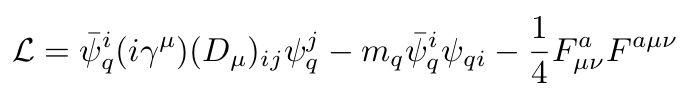
\includegraphics[width = 0.5\linewidth]{plots/part1/intro/qcd_lagrangian.png}
	\end{figure}

		QCD is the theory of the strong interactions $\longrightarrow$ interactions between {\color{red} quarks and gluons}
		
\end{frame}

% QCD and the strong interactions
\begin{frame}

	\frametitle{Introduction}
	\framesubtitle{QCD and the strong interactions}
	
	\footnotesize
	
	How to explore proton's inner structure?

	\begin{figure}
		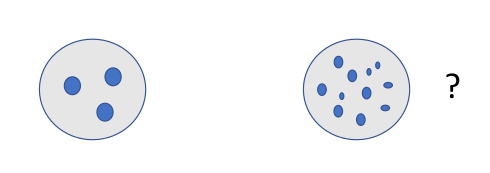
\includegraphics[width = 0.5\linewidth]{plots/part1/intro/protons.png}
	\end{figure}
	
	
	\begin{itemize}
		\item At different scales, hadrons show different behavior
		\item From point-like objects to complex internal dynamics
		\item Scattering experiments (DIS) and hadronic physics (LHC)
	\end{itemize}
	
	{\color{blue} \footnotesize "A way of describing high energy collisions is to consider any hadron as a composite object of point-like constituents $\longrightarrow$ \textbf{partons"} } R.Feynman, 1969 

\end{frame}

% Asymptotic freedom and pQCD
\begin{frame}

	\frametitle{QCD and collider physics}
	\framesubtitle{Asymptotic freedom and pQCD}

	\footnotesize
	
	\begin{columns}	
		
		\column{0.3\textwidth}
		
		\begin{figure}

			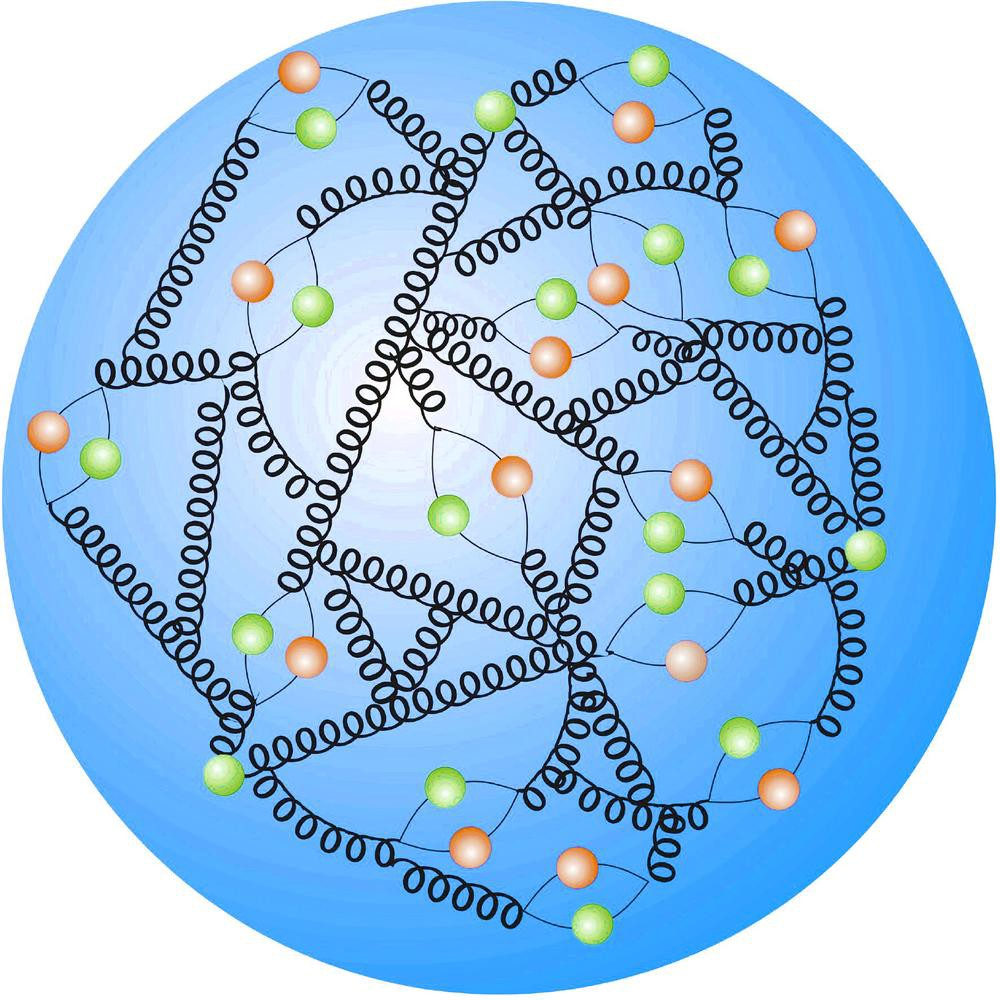
\includegraphics[width = 2 cm]{plots/part1/intro/proton2.jpg}
		\end{figure}
		
		\column{0.7\textwidth}
		
		\begin{itemize}
			\item Parton model as LO approximation to QCD
			\item QCD coupling strength $\alpha_{s}$ changes with energy
			\item At high energies the hadron involves extremely complex internal dynamics
		\end{itemize}
		
	\end{columns}
	
	\vspace{1cm}
	\center \footnotesize QCD is strongly coupled at large distances / low energies $\longrightarrow$ confinement
	\center \footnotesize \color{red} Non-perturbative physics

\end{frame}

%Asymptotic freedom and pQCD
\begin{frame}
	
	\frametitle{QCD and collider physics}
	\framesubtitle{Asymptotic freedom and pQCD}
	
	\footnotesize
	
	\begin{itemize}
		\item Running coupling given by Renormalization Group Equation (RGE)
		\begin{equation}
		{\color{blue}\mu\frac{d\alpha_{s}(\mu)}{d\mu} = \beta(\alpha_{s}(\mu)) = -\sum_{n = 0}^{\infty} \beta_{n} \Big( \frac{\alpha_{s}}{\pi} \Big)^{n + 1}} \nonumber
		\end{equation}
		\item Coupling {\color{blue}$\alpha_{s}$} evolves with scale {\color{blue}$\mu$} as given by RGE $\rightarrow$ LO behavior driven by $\beta_{0}$
		\item Main difference between QED and QCD
		\begin{itemize}
			\item $\beta_{0}^{\textrm{QED}} < 0 \implies$ strongly coupled at large energies
			\item $\beta_{0}^{\textrm{QCD}} > 0 \implies$ weakly coupled at large energies
		\end{itemize}
	\end{itemize}

\end{frame}

% Asymptotic freedom and pQCD
\begin{frame}

	\frametitle{QCD and collider physics}
	\framesubtitle{Asymptotic freedom and pQCD}
	
	\begin{columns}	
		
		\column{0.5\textwidth}
		
		\begin{figure}
			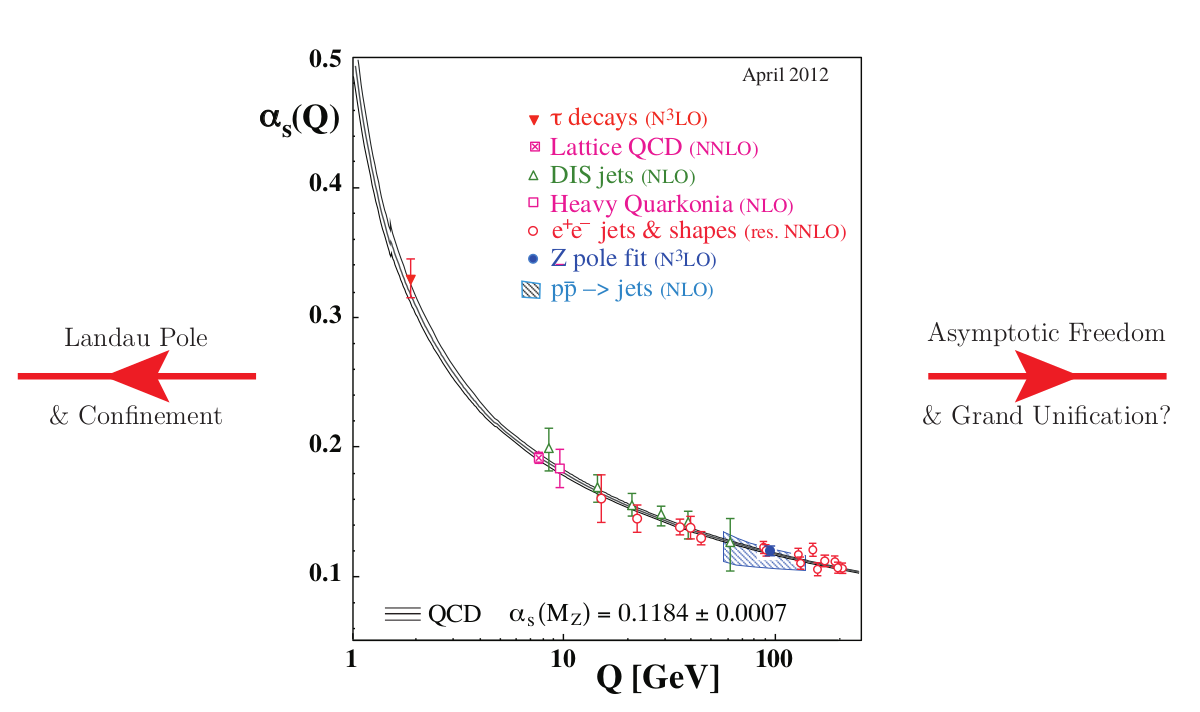
\includegraphics[width = 6 cm]{plots/part1/chapter1/qcd_running_fit.png}
		\end{figure}
		
		\column{0.5\textwidth}
		
		\begin{itemize}
			\item \footnotesize Running coupling given by Renormalization Group Equation (RGE)
			\begin{equation}
			\alpha_{s}(\mu) = \frac{1}{\beta_{0} \log\big( \frac{\mu^{2}}{\Lambda_{\textrm{QCD}}^{2}}\big)} \nonumber
			\end{equation}
			\item \footnotesize $\beta_{0}$ LO of the $\beta$ function, is $ > 0$
			\item \footnotesize $\Lambda_{\textrm{QCD}}$, parameter that defines value \\ of the coupling at large scales
		\end{itemize}
		
	\end{columns}
	
	\vspace{1cm}
	\center \footnotesize QCD is weakly coupled for $\mu >> \Lambda_{\textrm{QCD}} \longrightarrow$ asymptotically free
	\center \footnotesize \color{red} Perturbative Quantum Chromodynamics (pQCD)

\end{frame}

% Hadronic processes and factorization
\begin{frame}
	
	\frametitle{QCD and collider physics}
	\framesubtitle{Hadronic processes and factorization}
	
	\footnotesize
	
	\vspace{0.4 cm}
	
	\begin{figure}
		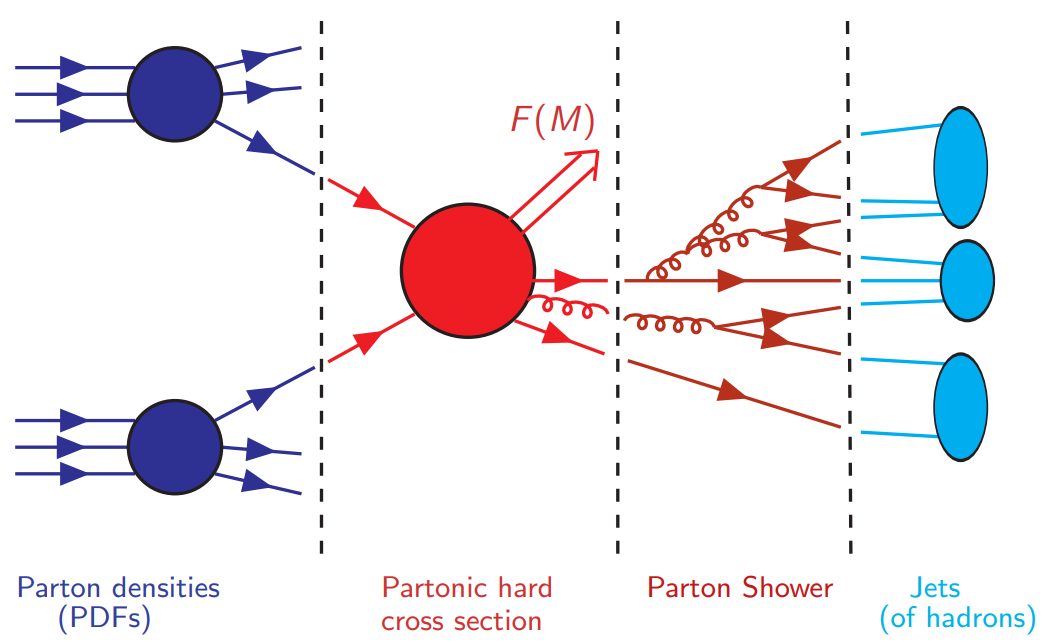
\includegraphics[width = 7 cm]{plots/part1/chapter2/factorization_1.png}
	\end{figure}
	
	\begin{itemize}
		\item LHC physics rely on hadronic collisions $\longrightarrow$ pQCD
		\item Compute \textbf{cross section} $\sigma^{F}$ $\longrightarrow$ probability for a given process
	\end{itemize}

\end{frame}

% Hadronic processes and factorization
\begin{frame}

	\frametitle{QCD and collider physics}
	\framesubtitle{Hadronic processes and factorization}
	
	\footnotesize
	
	\vspace{0.4 cm}
	
	\begin{figure}
		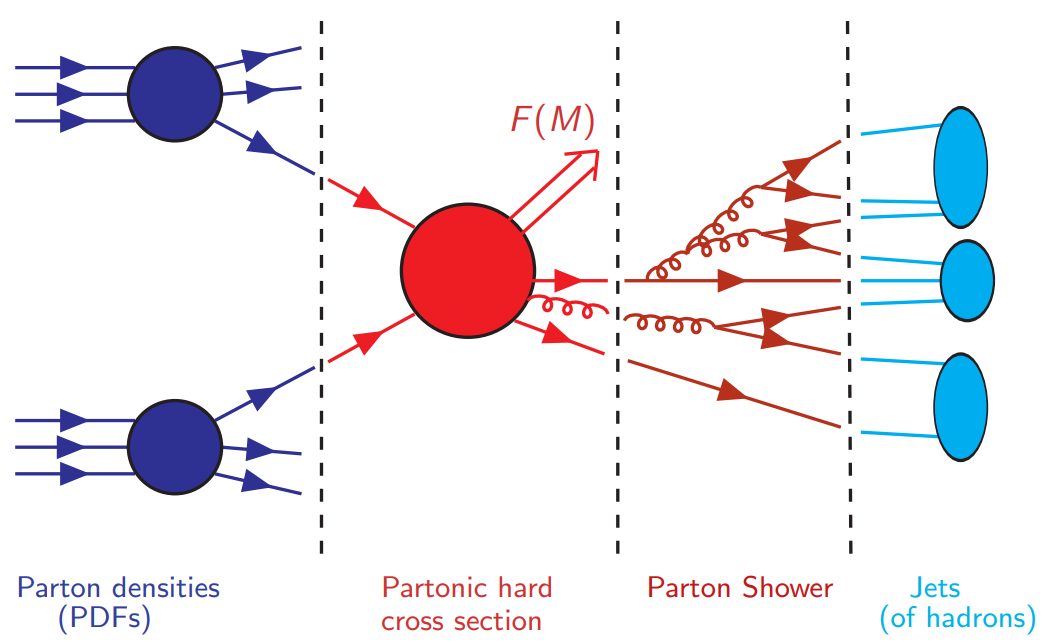
\includegraphics[width = 7 cm]{plots/part1/chapter2/factorization_1.png}
	\end{figure}
	
	Compute hadronic cross sections is a {\color{red}hard problem} $\longrightarrow$ {\color{blue} QCD Factorization}
	
	\begin{equation}
		\sigma^{\textrm{F}}(p_{1}, p_{2}) =
		\int_{0}^{1} dx_{1} dx_{2} \; {\color{blue} f_{\alpha}(x_{1}, \mu_{F}^{2}) \ast f_{\beta}(x_{2}, \mu_{F}^{2})}
		\; \ast \;  
		{\color{red}\hat{\sigma}^{\textrm{F}}_{\alpha \beta}(x_{1}p_{1}, x_{2}p_{2}, \alpha_{s}(\mu_{R}^{2}), \mu_{F}^{2})} \nonumber
	\end{equation}

\end{frame}

% Hadronic processes and factorization
\begin{frame}

	\frametitle{QCD and collider physics}
	\framesubtitle{Hadronic processes and factorization}
	
	\footnotesize
	
	\begin{figure}
		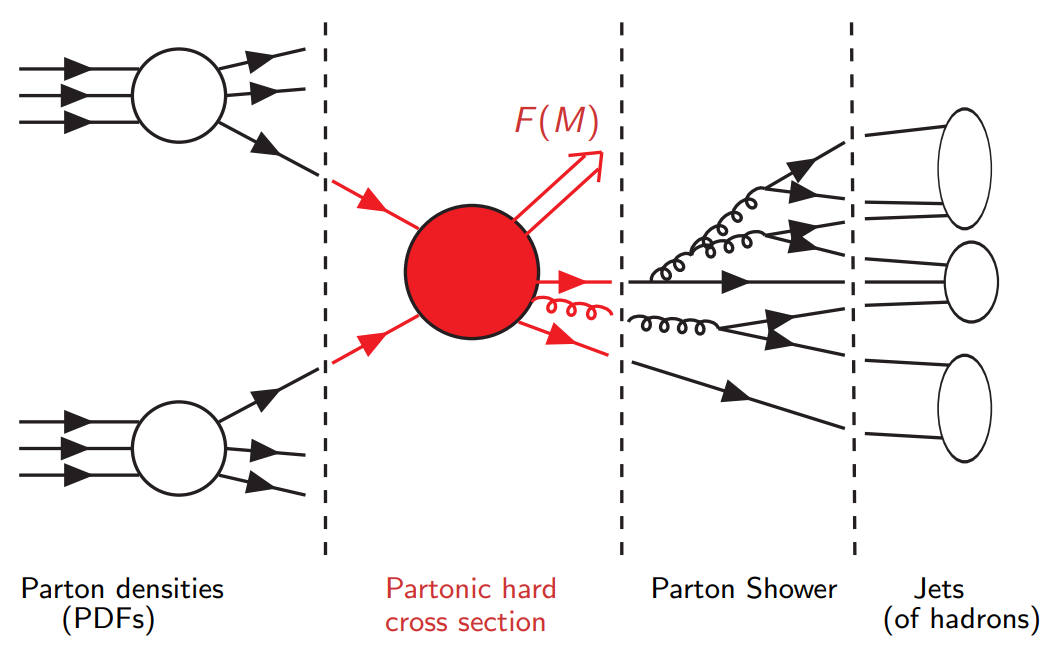
\includegraphics[width = 7 cm]{plots/part1/chapter2/factorization_2.png}
	\end{figure}
	
	\begin{itemize}
		\item Parton densities (PDFs) ${\color{blue} f_{\alpha}(x_{i}, \mu_{F}^{2})}$: non perturbative but universal
		\item Partonic cross section {\color{red}$\hat{\sigma}^{\textrm{F}}_{\alpha \beta}$}: process dependent but computable as perturbative series in $\alpha_{s}$
	\end{itemize}

\end{frame}

% Parton densities
\begin{frame}
	
	\frametitle{QCD and collider physics}
	\framesubtitle{Parton densities}
	
	\footnotesize

	\begin{columns}
	
	\column{0.5\textwidth}

	{\color{blue} Parton Distribution Functions: probability distribution of finding a particular parton \\ (u, d, ..., g) carrying a fraction x of the proton's momentum}

	\column{0.3\textwidth}
	
	\begin{figure}
		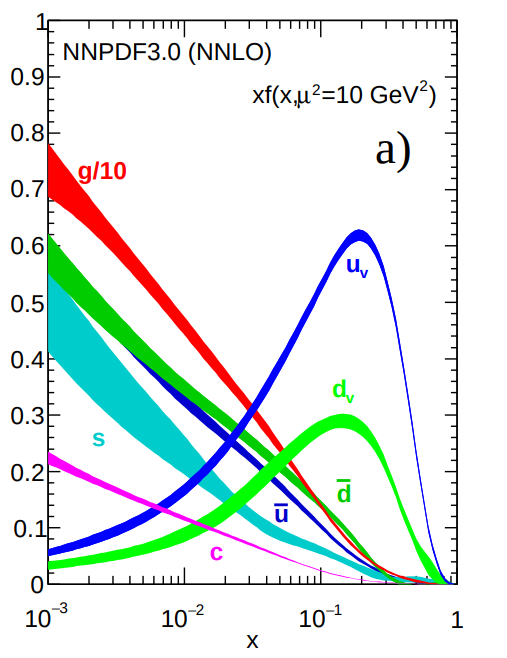
\includegraphics[width = 3 cm]{plots/part1/chapter2/PDF.png}
	\end{figure}
	
	\end{columns}

	\begin{itemize}
		\item Each parton has a different PDF $\longrightarrow$ ${\color{blue}u(x)}, {\color{green}d(x)}, ..., {\color{red}g(x)}$
		\item PDFs can not predicted and yet can not measured $\longrightarrow$ extracted from data \\ (MSTW, CTEQ, NNPDF collaborations)
		\item The N3PDF project: Machine Learning for PDFs determination
	\end{itemize}

\end{frame}

% The N3PDF project
\begin{frame}
	
	\frametitle{QCD and collider physics}
	\framesubtitle{The N3PDF project}
	
	\footnotesize
	
	\begin{figure}[!htb]
		\minipage{0.32\textwidth}
		
\includegraphics[width = 0.5\linewidth]{plots/backup/TF.png}
		\endminipage\hfill
		\minipage{0.5\textwidth}
		
\includegraphics[width = 0.5\linewidth]{plots/backup/Keras.png}
		\endminipage\hfill
	\end{figure}
	
	\begin{itemize}
		\item Use \texttt{TensorFlow} and \texttt{Keras} to determine the PDFs with ML fitting models
		\item See paper by S.Carrazza - J.Cruz-Martinez \\
		{\color{blue}"Towards a new generation of parton densities with deep learning models",\\
		Carrazza et al., https://arxiv.org/abs/1907.05075}
		\item TensorFlow operator implementation $\longrightarrow$ optimize PDF fitting \\
		{\color{blue}"Towards hardware acceleration for parton densities estimation",\\ Urtasun-Elizari et al., https://arxiv.org/abs/1909.10547}
	\end{itemize}

\end{frame}

% The N3PDF project
\begin{frame}
	
	\frametitle{QCD and collider physics}
	\framesubtitle{General structure of n3fit}
	
	\footnotesize
	
	\begin{figure}
		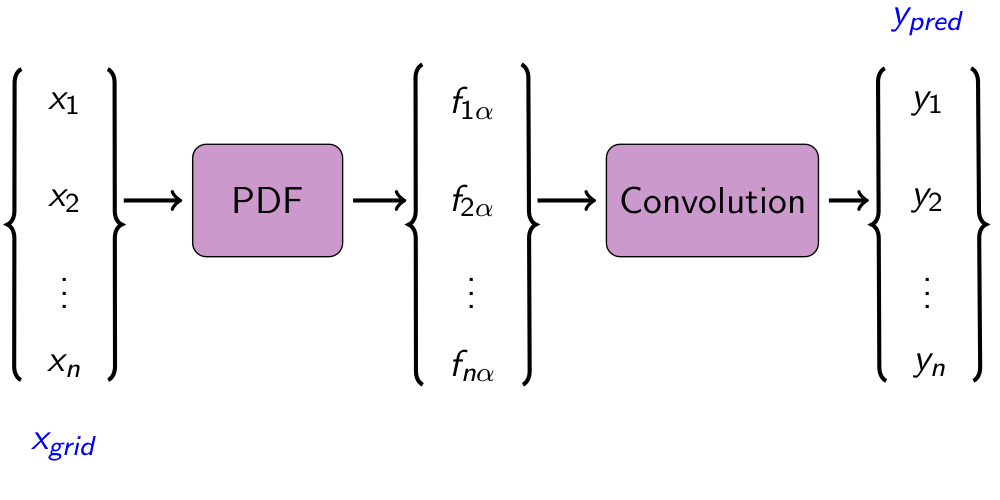
\includegraphics[width = 9 cm]{plots/backup/n3fit1.png}
	\end{figure}	
	
	\begin{enumerate}
		\item Build a NN to compute $y_{pred}$ observables from a grid of momentum fractions $x_{i}$
		\item Compute $\chi^{2}$ loss function by comparing with LHC data
		\item Update values of PDF through $\chi^{2}$ minimization $\longrightarrow$ {\color{violet} Fit}
	\end{enumerate}
	
	\end{frame}

% The N3PDF project
\begin{frame}
	
	\frametitle{QCD and collider physics}
	\framesubtitle{Operator implementation in TF}
	
	\footnotesize
	
	\begin{figure}
	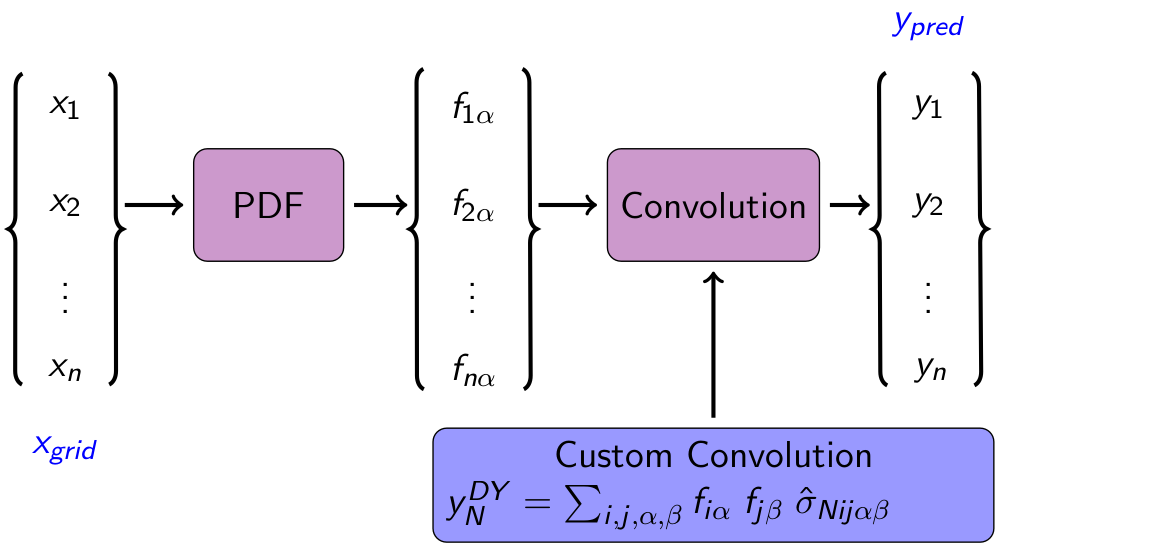
\includegraphics[width = 10.5 cm]{plots/backup/n3fit2.png}
	\end{figure}
	
	\begin{enumerate}
	\item TF relies in symbolic computation $\longrightarrow$ High memory usage
	\item Implement \texttt{C++} operator replacing the convolution
	\item {\color{blue}[Urtasun-Elizari et al.]} ref. at {\color{blue} \href{https://arxiv.org/abs/1910.07049}{1910.07049}}
\end{enumerate}

\end{frame}

% Partonic cross section and pQCD
\begin{frame}
	
	\frametitle{QCD and collider physics}
	\framesubtitle{Partonic cross section and pQCD}
	
	\footnotesize
	
	\begin{columns}
	
	\column{0.5\textwidth}
	
	\begin{itemize}
		\item Born cross section is the leading-order (LO) term of the perturbative series
		\item $\sigma^{(1)}, \sigma^{(2)}, \sigma^{(3)}$ are the NLO, NNLO, N$^{3}$LO corrections
	\end{itemize}
	
	\column{0.45\textwidth}
	
	\begin{figure}[!htb]
		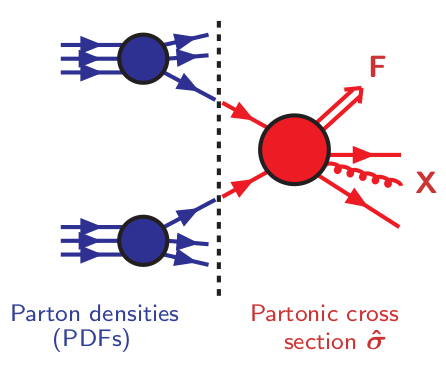
\includegraphics[width = 5 cm]{plots/part1/chapter2/factorization_3.png}
	\end{figure}
	
	\end{columns}
	
	\begin{equation}
		\hat{\sigma} = \sigma^{\texttt{Born}} \Big( 1 +
		\alpha_{s} \sigma^{(1)} + 
		\alpha_{s}^{2} \sigma^{(2)} + 
		\alpha_{s}^{3} \sigma^{(3)} + ... \Big) \nonumber
	\end{equation}
	
	\footnotesize Lower order predictions strongly depend on the auxiliary / unphysical scales \\ {\color{red}Need higher order corrections to increase theoretical accuracy!}

\end{frame}

% LHC physics
\begin{frame}
	
	\frametitle{QCD and collider physics}
	\framesubtitle{LHC phenomenology}
	
	\begin{figure}
		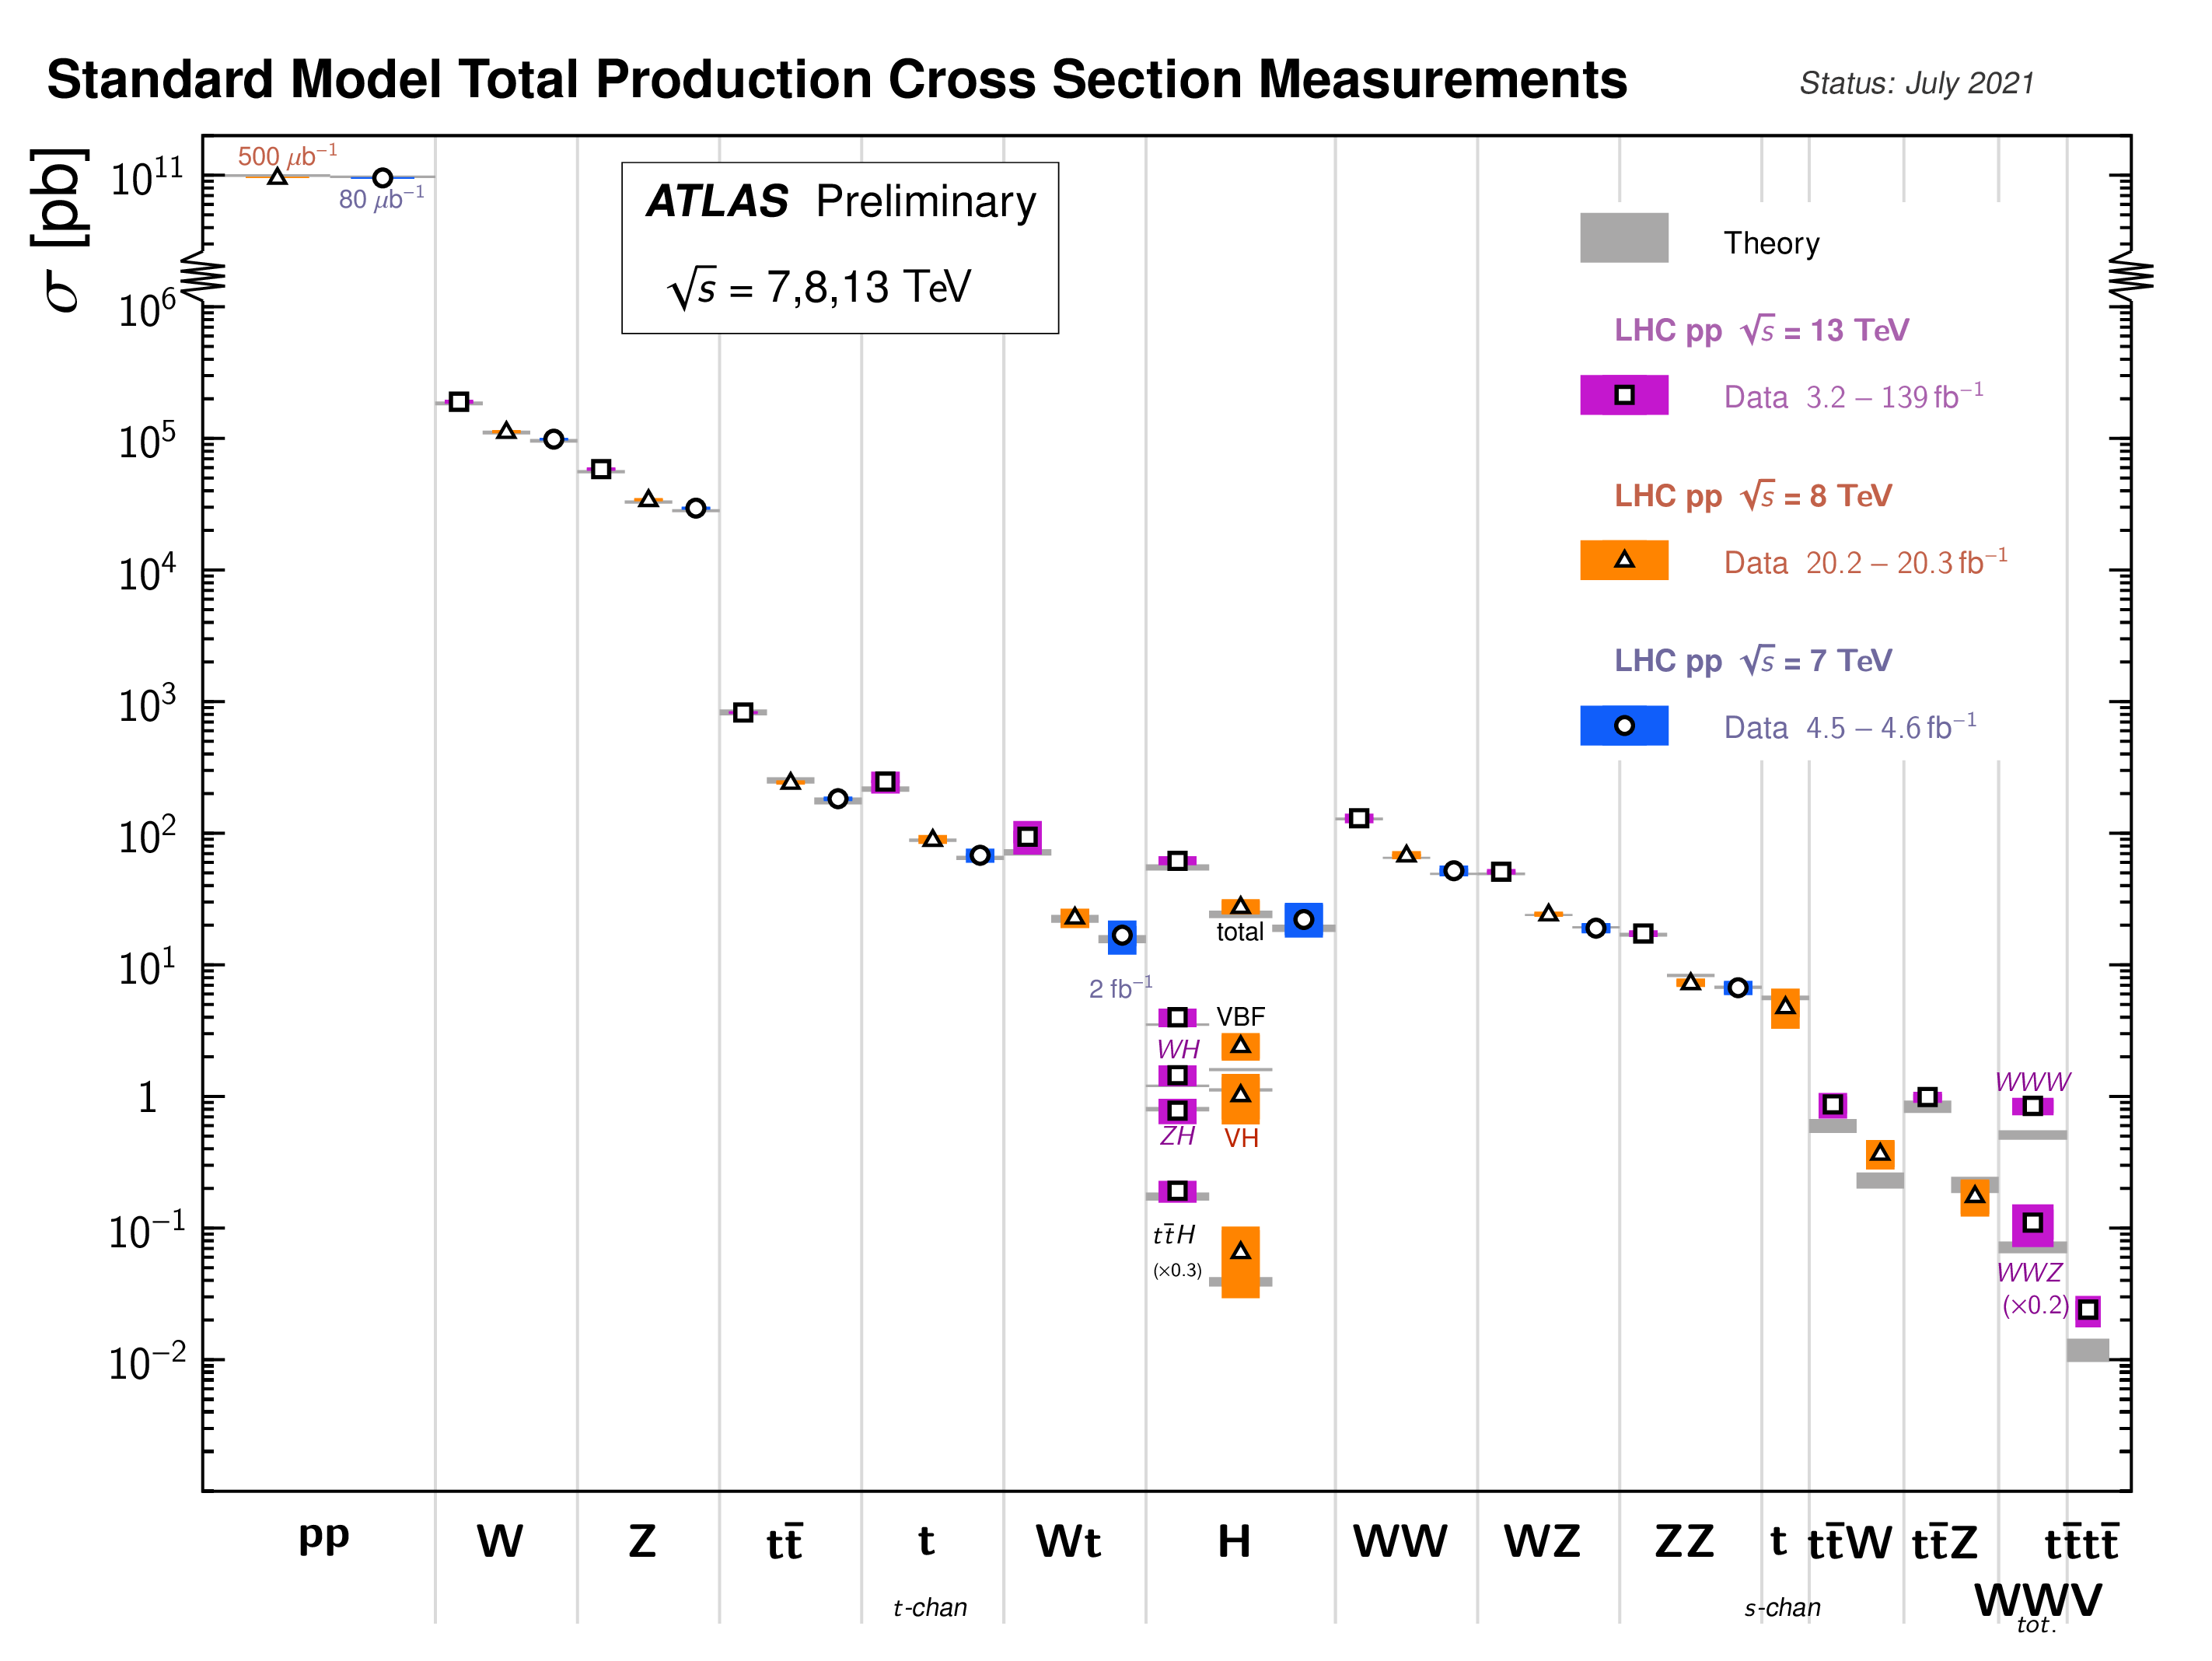
\includegraphics[width = 8.5 cm]{plots/part1/chapter3/lhc_measurements.png}
	\end{figure}
		
\end{frame}

%
% Part 2 .................................................................................
% All order resummation ..................................................................
%

% Dealing with divergences
\begin{frame}

	\center{\color{blue}Part II \\ All order resummation}

\end{frame}

% Higher order corrections
\begin{frame}

	\frametitle{Resummation in QCD}
	\framesubtitle{Higher order corrections - need for resummation}

	\footnotesize
	
	\begin{columns}
	
	\column{0.5\textwidth}
	
	\begin{enumerate}
		\item Calculation of higher order corrections is {\color{red}not an easy task} due to {\color{red} infrared (IR) soft and collinear singularities}
		\item Final state singularities {\color{blue}cancel} by combining real and virtual contributions $\longrightarrow$ KLN theorem
		\item Initial state collinear singularities {\color{blue}factorized} inside the PDFs
	\end{enumerate}
	
	\column{0.45\textwidth}
	\begin{figure}[!htb]
		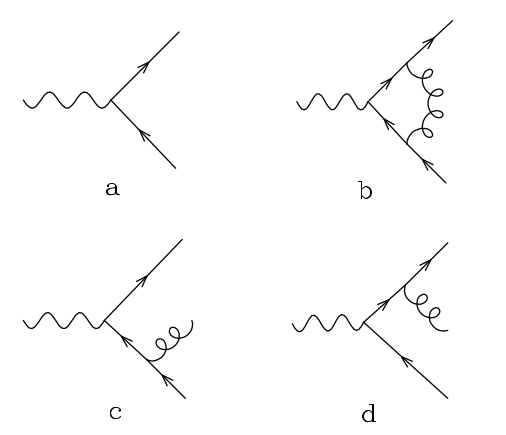
\includegraphics[width = \linewidth]{plots/part2/qcd_corrections.png}
	\end{figure}
	
	\end{columns}

	\vspace{0.5 cm}
	
	Complete cancellation only works in inclusive final states!

\end{frame}

% qT resummation I
\begin{frame}

	\frametitle{Resummation in QCD}
	\framesubtitle{$q_{\perp}$ resummation}
	
	\footnotesize
	
	\begin{columns}
	
		\column{0.55\textwidth}
		
		\begin{itemize}
			\item Describing exclusive final states \\
			\item Study the differential $q_{\perp}$ distribution \\
			$h_{1}(p_{1}) + h_{2}(p_{2}) \longrightarrow F(M, {\color{red}q_{\perp}}) + X$
		\end{itemize}
		
		\column{0.45\textwidth}
		
		\begin{figure}
			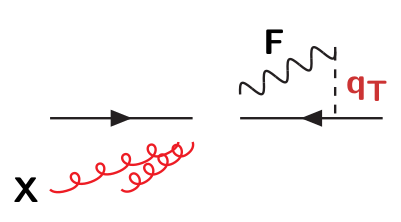
\includegraphics[width = 4cm]{plots/part2/qT_diagram.png}
		\end{figure}

	\end{columns}
 
	$\int_{0}^{Q_{\perp}^{2}} \; dq_{\perp}^{2} \frac{d\hat{\sigma}}{dq_{\perp}^{2}} \sim c_{0} + \alpha_{s}(c_{12}L^{2} + c_{11}L + c_{10}) + ..., \textrm{\quad where \quad} L = \ln (M^{2} / q_{\perp}^{2})$

	\begin{figure}
		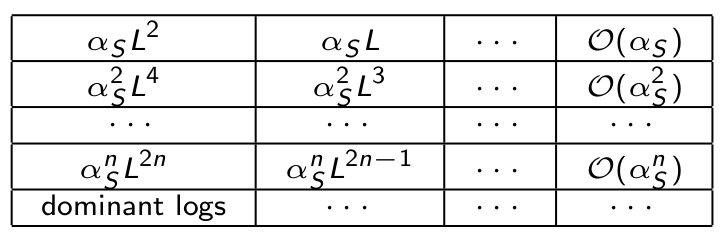
\includegraphics[width = 7cm]{plots/part2/qT_logs_table.png}
	\end{figure}

	Truncated fixed-order predictions $\rightarrow$ {\color{red}enhanced $\alpha_{s}^{n}\ln^{m}(M^{2}/q_{\perp}^{2})$ appear}

\end{frame}

% Resummation in QCD II
\begin{frame}

	\frametitle{Resummation in QCD}
	\framesubtitle{$q_{\perp}$ resummation}

	\footnotesize
	
	\begin{itemize}
		\item Catani - Bozzi - de Florian - Grazzini (CBFG) formalism (*) \\
		{\color{blue}"Transverse-momentum resummation and the spectrum\\
			of the Higgs boson at the LHC",\\
		Bozzi et al., https://arxiv.org/abs/hep-ph/0508068}
		\item Separate partonic $q_{\perp}$ distribution as follows:
	\end{itemize}
	
	\begin{equation}
		\frac{d\hat{\sigma}_{ab}}{dq_{\perp}^{2}} =
		\Bigg[ \frac{d\hat{\sigma}^{\textrm{(res.)}}_{ab}}{dq_{\perp}^{2}} \Bigg]_{\textrm{l.a.}} + 
		\Bigg[ \frac{d\hat{\sigma}^{\textrm{(fin.)}}_{ab}}{dq_{\perp}^{2}} \Bigg]_{\textrm{f.o.}} \textrm{\quad, \quad such that} \nonumber
	\end{equation}

	\begin{align}
		\int_{0}^{q_{\perp}^{2}} dq_{\perp}^{2} \frac{d\hat{\sigma}^{\textrm{(res.)}}_{ab}}{dq_{\perp}^{2}} \sim & \sum \alpha_{s}^{n} \log^{m} \bigg( \frac{M^{2}}{q_{\perp}^{2}} \bigg) \textrm{\quad for \quad} q_{\perp} \rightarrow 0 \nonumber \\
		\lim_{q_{\perp} \rightarrow 0}\int_{0}^{q_{\perp}^{2}} dq_{\perp}^{2} \frac{d\hat{\sigma}^{\textrm{(fin.)}}_{ab}}{dq_{\perp}^{2}} &= 0 \nonumber 
	\end{align}

	Resummed and finite components can be matched (LL+LO, NLL+NLO,\\ NNLO+NNLL, ...) to have uniform accuracy in a wide range of $q_{\perp}$
	
\end{frame}

% qT resummation III
\begin{frame}

	\frametitle{Resummation in QCD}
	\framesubtitle{Resummed component}
	
	\footnotesize
	
	Resummation holds in impact parameter space $b$
	
	\begin{equation}
		\frac{d\hat{\sigma}_{ab}^{\textrm{(res.)}}}{dq_{\perp}^{2}} = \frac{M^{2}}{\hat{s}} \int db \; \frac{b}{2} \; J_{0}(b q_{\perp}) \; {\color{red} \mathcal{W}_{ab}(b, M)} \nonumber
	\end{equation}
	 
	with ${\color{red}\mathcal{W}_{ab}}$ also expressed in Mellin space (with respect to $z = M^{2}/\hat{s}$)
	\begin{equation}
		{\color{red} \mathcal{W}_{N}(b, M) = \mathcal{H}_{N}(\alpha_{s}) \times \exp\{\mathcal{G}_{N}(\alpha_{s}, L)\}} \quad\textrm{being}\quad L \equiv \log(M^{2}b^{2}) \nonumber
	\end{equation}

	\begin{itemize}
		\item Large logarithms exponentiated in the universal Sudakov form factor {\color{red}$\mathcal{G}_{N}(\alpha_{s}, L)$}
		\item Constant (b-independent) terms factorized in the process dependent hard factor {\color{red}$\mathcal{H}_{N}(\alpha_{s})$}
	\end{itemize}
	
\end{frame}

% Extend formalism to N3LL
\begin{frame}

	\frametitle{Resummation in QCD}
	\framesubtitle{Extend formalism to N$^{3}$LL}
	
	\footnotesize
	
	Sudakov factor $\mathcal{G}_{N}$ and hard coefficient $\mathcal{H}_{N}$ can be expanded as perturbative series in $\alpha_{s}$
	\begin{align}
		\mathcal{G}_{N}(\alpha_{s}, L) &= L\;g^{(1)}(\alpha_{s}L) + g^{(2)}(\alpha_{s}L) + \frac{\alpha_{s}}{\pi}g^{(3)}(\alpha_{s}L) + {\color{red} \bigg( \frac{\alpha_{s}}{\pi} \bigg) ^{2}g^{(4)}(\alpha_{s}L)} + ... \nonumber \\
		\mathcal{H}_{N}(\alpha_{s}) &= 1 + \alpha_{s}\mathcal{H}^{(1)} + \alpha_{s}^{2}\mathcal{H}^{(2)} + {\color{red}\alpha_{s}^{2}\mathcal{H}^{(3)}} + ...  \nonumber
	\end{align}
	
	For each new order implement a factor of $\mathcal{G}_{N}$ and Hard $\mathcal{H}_{N}$
	
	\begin{columns}
		
		\column{0.45\textwidth}
		
		\begin{align}
			&\textrm{LL} (\sim \alpha_{s}^{n}L^{n+1}): g^{(1)}, \hat{\sigma}^{(0)} \nonumber \\
			&\textrm{NLL} (\sim \alpha_{s}^{n}L^{n}): g^{(2)}, \mathcal{H}^{(1)} \nonumber \\
			&\textrm{NNLL} (\sim \alpha_{s}^{n}L^{n-1}): g^{(3)}, \mathcal{H}^{(2)} \nonumber \\
			&{\color{red} \textrm{N$^{3}$LL} (\sim \alpha_{s}^{n}L^{n-2}): g^{(4)}, \mathcal{H}^{(3)}} \nonumber
		\end{align}
		
		\column{0.45\textwidth}
		
		\begin{itemize}
			\item Implement CBFG resummation \\ 
			in \texttt{C++} code
			\item Extend the formalism up to {\color{red}N$^{3}$LO+N$^{3}$LL} accuracy!
		\end{itemize}
	
	\end{columns}

\end{frame}

%
% Part 3 .................................................................................
% HTurbo numerical implementation ........................................................
%

% Part 3
\begin{frame}

	\center{\color{blue}Part III \\ HTurbo numerical implementation}

\end{frame}

% Resummation for Higgs differential distribution
\begin{frame}
	
	\frametitle{HTurbo}
	\framesubtitle{Resummation for Higgs differential distribution}

	\footnotesize
	
	\begin{itemize}
		\item Fast and accurate predictions for Higgs boson production cross section
		\item Predictions for differential cross section $d\sigma^{\textrm{H}} / dq_{\perp}^{2}$
		\item Numerical implementation of resummed and finite components
	\end{itemize}

	\begin{columns}
		
		\column{0.5\textwidth}

		\begin{align}
			d\sigma^{\textrm{H}}_{\textrm{(N)NLL+(N)LO}} &= 
			d\sigma^{\textrm{(res.)}}_{\textrm{(N)NLL}} - 
			d\sigma^{\textrm{(asy.)}}_{\textrm{(N)LO}} + 
			d\sigma^{\textrm{(f.o.)}}_{\textrm{(N)LO}} \nonumber \\
			d\sigma^{\textrm{(res.)}}_{\textrm{(N)NLL}} &= \hat{\sigma}^{\textrm{H}}_{\textrm{LO}} \times \mathcal{H}_{\textrm{(N)LO}} \times \exp{\mathcal{G}}_{\textrm{(N)NLL}} \; \nonumber \\
			d\sigma^{\textrm{(asy.)}}_{\textrm{(N)LO}} &= \hat{\sigma}^{\textrm{H}}_{\textrm{LO}} \times \Sigma_{\textrm{(N)LO}} \nonumber
		\end{align}
	
		\column{0.5\textwidth}
		
		\begin{figure}
			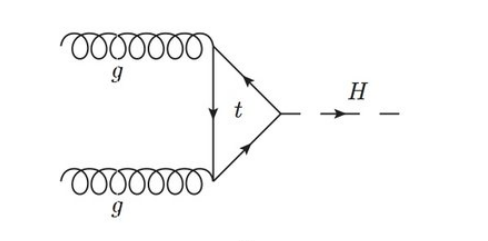
\includegraphics[width = 5 cm]{plots/part3/chapter5/higgs.png}
		\end{figure}	
		
	\end{columns}

	\begin{itemize}
		\item LO process is just gg $\rightarrow$ H, but NLO and beyond require gg $\rightarrow$ H + jet!
	\end{itemize}

\end{frame}

% HqT and HRes
\begin{frame}

	\frametitle{HTurbo}
	\framesubtitle{Predictions for Higgs $q_{\perp}$ distribution}
	
	\footnotesize
	
	\begin{columns}
		
		\column{0.5\textwidth}
			
		\begin{itemize}
			\item $q_{\perp}$ resummation implemented in numerical codes \textbf{HqT}, \textbf{HRes}, \textbf{HNNLO} {\color{blue}[Catani, de Florian, \\ Ferrera, Grazzini, Tommasini]} 
			\item Higher order accuracy require \\
			{\color{red}high computation times}
			\item NNLL predictions can take \\ more than 48h {\color{red} just for 1 PDF set \\
			and 1 $\mu_{R}, \mu_{F}$ value} $\longrightarrow$ need for \\ {\color{red} fast numerical implementations}
		\end{itemize}

		\column{0.45\textwidth}
	
		\begin{figure}
			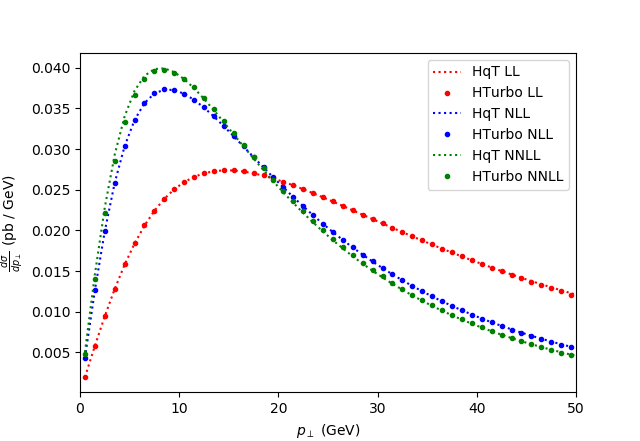
\includegraphics[width = 6 cm]{plots/part3/chapter6/higgs_qt_all.png}
		\end{figure}		
			
	\end{columns}

	\vspace{0.5 cm}
	
	Codes producing fast and accurate predictions are needed for precision era of the LHC \\
	(High Luminosity LHC, from 80 - 140 fb$^{-1}$ to \textbf{2000 fb$^{-1}$} !)
	
\end{frame}

% DYturbo I
\begin{frame}

	\frametitle{HTurbo}
	\framesubtitle{Starting point: DYTurbo}

	\footnotesize
	
	Numerical code \textbf{DYTurbo} {\color{blue}[Camarda et al., https://arxiv.org/abs/1910.07049]}, \\ fast and precise $q_{\perp}$ resummation and several improvements for Drell-Yan ($h_{1}h_{2} \rightarrow V + X \rightarrow l^{+}l^{-} + X$) 
	
	\vspace{0.5 cm}
	
	{\color{red}First goal}: set up a numerical code for Higgs boson production starting from  \textbf{DYTurbo}
 
	\begin{itemize}
		\item Set LO amplitude $gg \rightarrow H$
		\item Set Sudakov and Hard coefficients for resummed component
		\item Set $\Sigma$ coefficients for asymptotic term
		\item Implement MC producing the LO and NLO H+jet cross sections
		\item Compare with \textbf{HRes} and \textbf{HqT}
	\end{itemize}

	\vspace{0.2 cm}

	{\color{red}Final goal}: extend theoretical accuracy up to N$^{3}$LL+N$^{3}$LO

\end{frame}

% DYturbo II
\begin{frame}

	\frametitle{HTurbo}
	\framesubtitle{Code optimization}
	
	\footnotesize
	
	Optimized reimplementation of \textbf{HqT}, \textbf{HRes} and \textbf{HNNLO} for $q_{T}$-resummation
	
	\vspace{0.2 cm}
		
	\begin{itemize}
		\item \textbf{C++} structure with \textbf{Fortran} interfaces $\rightarrow$ Multi-threading
		\item Optimization in the integration routines / integral transforms 
		\begin{itemize}
			\item Factorize boson and decay kinematics
			\item Gauss-Legendre quadrature rules (1-dim.)
			\item Vegas/Cuhre through \textbf{Cuba} (multi-dim.)
		\end{itemize}
	\end{itemize}
	
	\vspace{0.5cm}
	
	Benchmark comparison with \textbf{HRes, HNNLO} - numerical and speed performance \\
	\begin{itemize}
		\item {\color{blue}"Higgs boson production at the LHC:
			fast and precise predictions in QCD at higher orders", Urtasun-Elizari et al., https://arxiv.org/abs/2202.10343}
	\end{itemize}
	
\end{frame}

% Results - Benchmark HRes - NLL resummed
\begin{frame}
	
	\frametitle{Results}
	\framesubtitle{Comparison HTurbo and HRes - NLL resummed}
	
	\footnotesize
	
	\begin{columns}
		
		\column{0.5\textwidth}
		
		\begin{figure}
			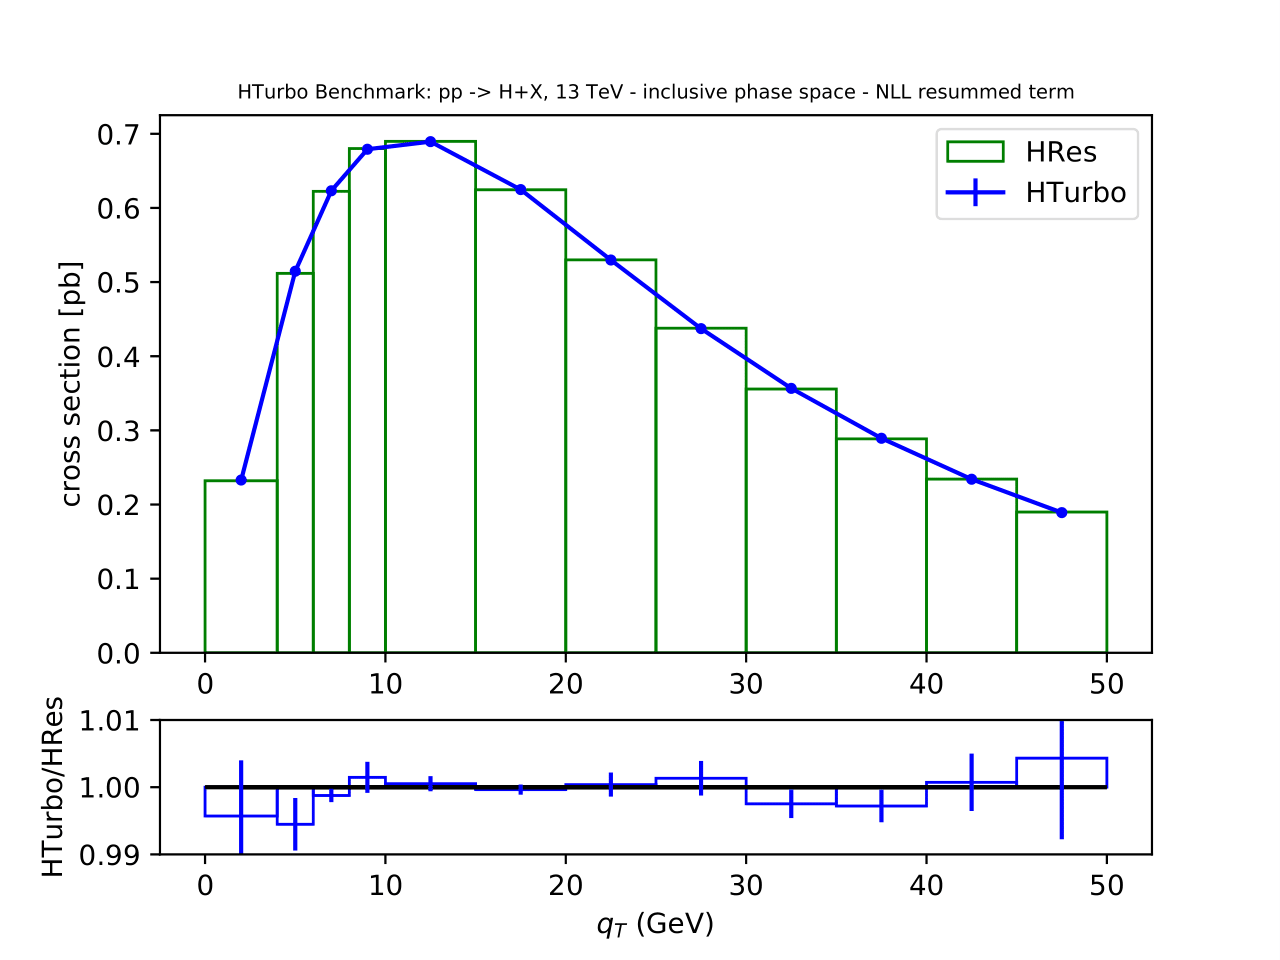
\includegraphics[width = 7cm]{plots/part3/chapter6/nlo-res-1.png}
		\end{figure}
		
		\column{0.5\textwidth}
		
		\begin{figure}
			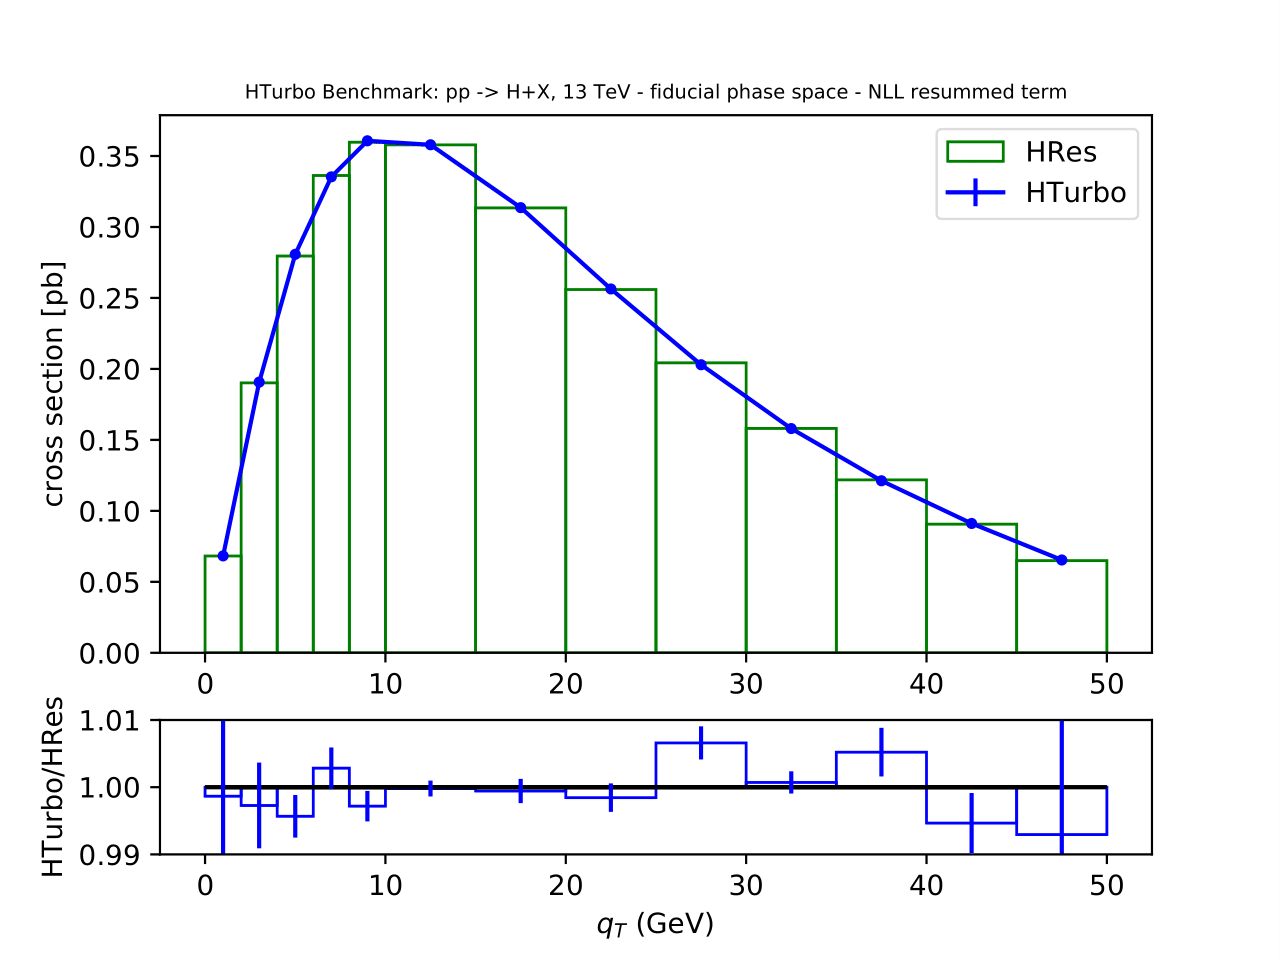
\includegraphics[width = 7cm]{plots/part3/chapter6/nlo-res-fid-1.png}
		\end{figure}
		
	\end{columns}
	
	\begin{itemize}
		\item Cross section for fully inclusive (LHS) and fiducial (RHS) phase space {\color{darkgreen}$\checkmark$} 
		\item CM energy $\sqrt s = 13$ GeV and PDF set \texttt{NNPDF31\_nlo\_as\_0118 PDF} set
	\end{itemize}

\end{frame}

% Results - Benchmark HRes - NNLL resummed
\begin{frame}
	
	\frametitle{Results}
	\framesubtitle{Comparison HTurbo and HRes - NNLL resummed}
	
	\footnotesize
	
	\begin{columns}
	
	\column{0.5\textwidth}
	
	\begin{figure}
		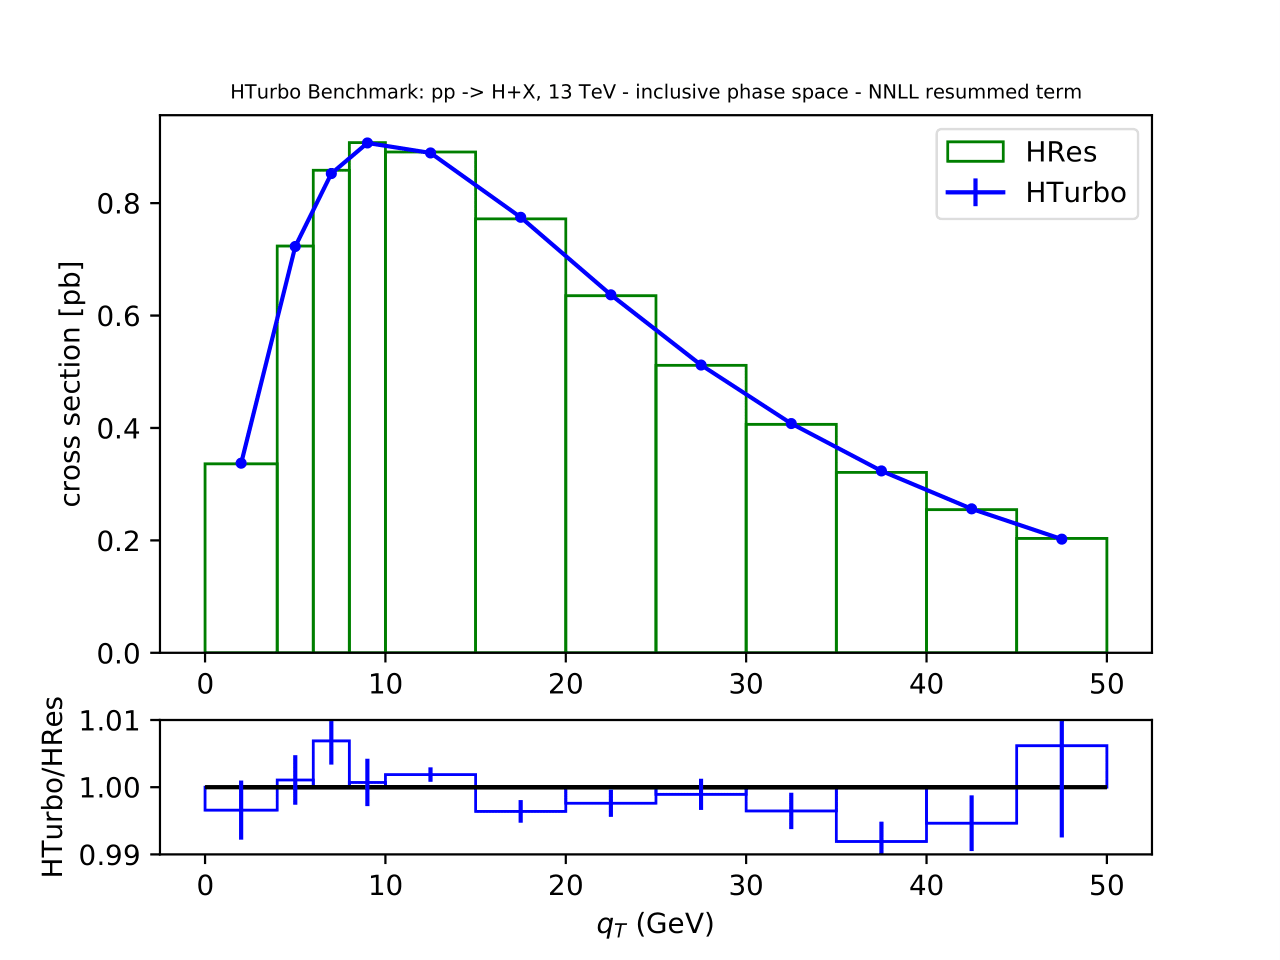
\includegraphics[width = 7cm]{plots/part3/chapter6/nnlo-res-1.png}
	\end{figure}
	
	\column{0.5\textwidth}
	
	\begin{figure}
		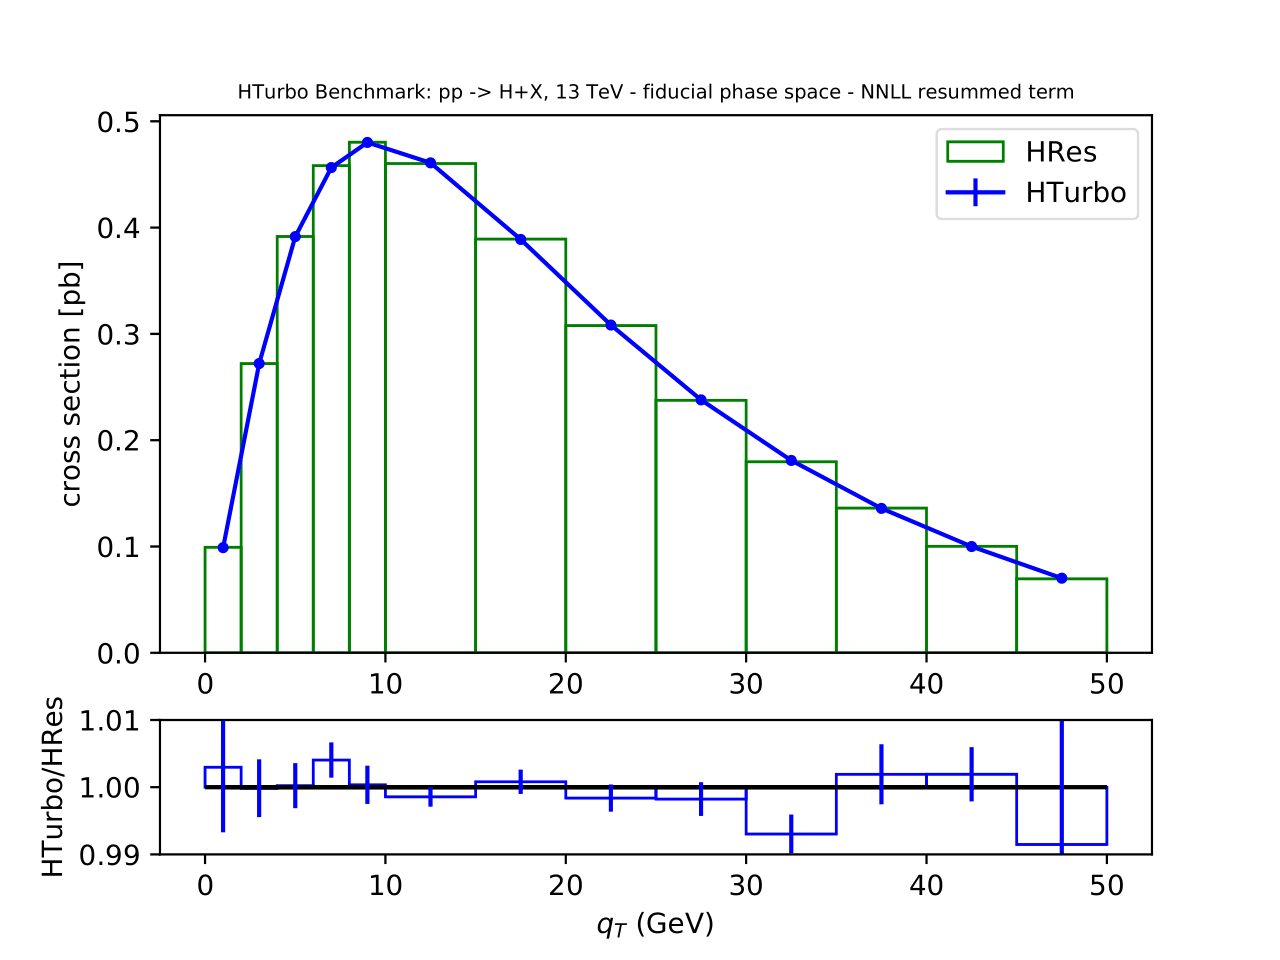
\includegraphics[width = 7cm]{plots/part3/chapter6/nnlo-res-fid-1.png}
	\end{figure}
	
	\end{columns}
	
	\begin{itemize}
	\item Cross section for fully inclusive (LHS) and fiducial (RHS) phase space {\color{darkgreen}$\checkmark$} 
	\item CM energy $\sqrt s = 13$ GeV and PDF set \texttt{NNPDF31\_nnlo\_as\_0118 PDF} set
	\end{itemize}

\end{frame}

% Results - Benchmark HRes - LO asymptotic
\begin{frame}
	
	\frametitle{Results}
	\framesubtitle{Comparison HTurbo and HRes - LO asymptotic}
	
	\footnotesize
	
	\begin{columns}
		
		\column{0.5\textwidth}
		
		\begin{figure}
			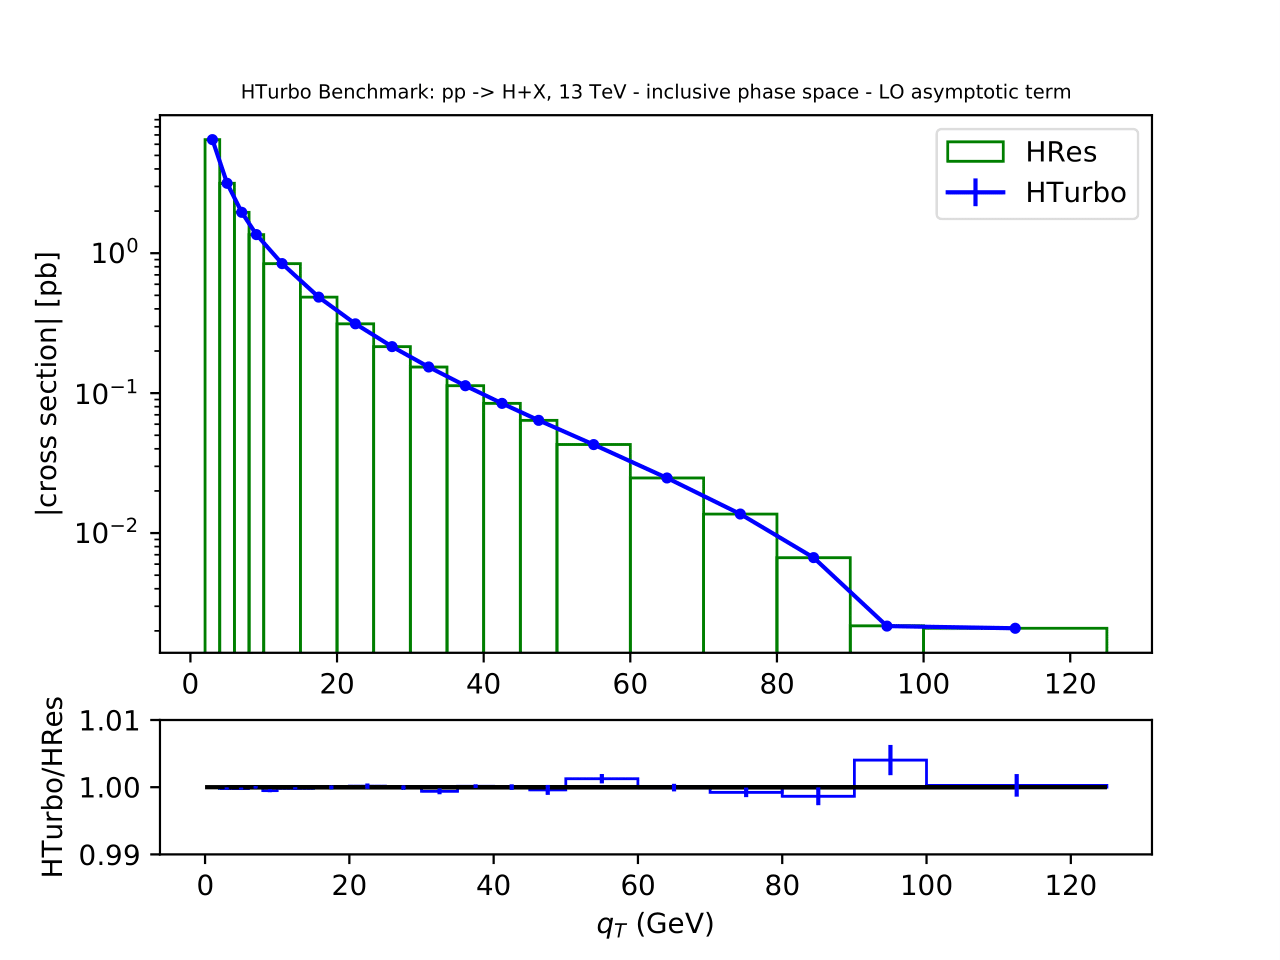
\includegraphics[width = 7cm]{plots/part3/chapter6/nlo-ct-1.png}
		\end{figure}
		
		\column{0.5\textwidth}
		
		\begin{figure}
			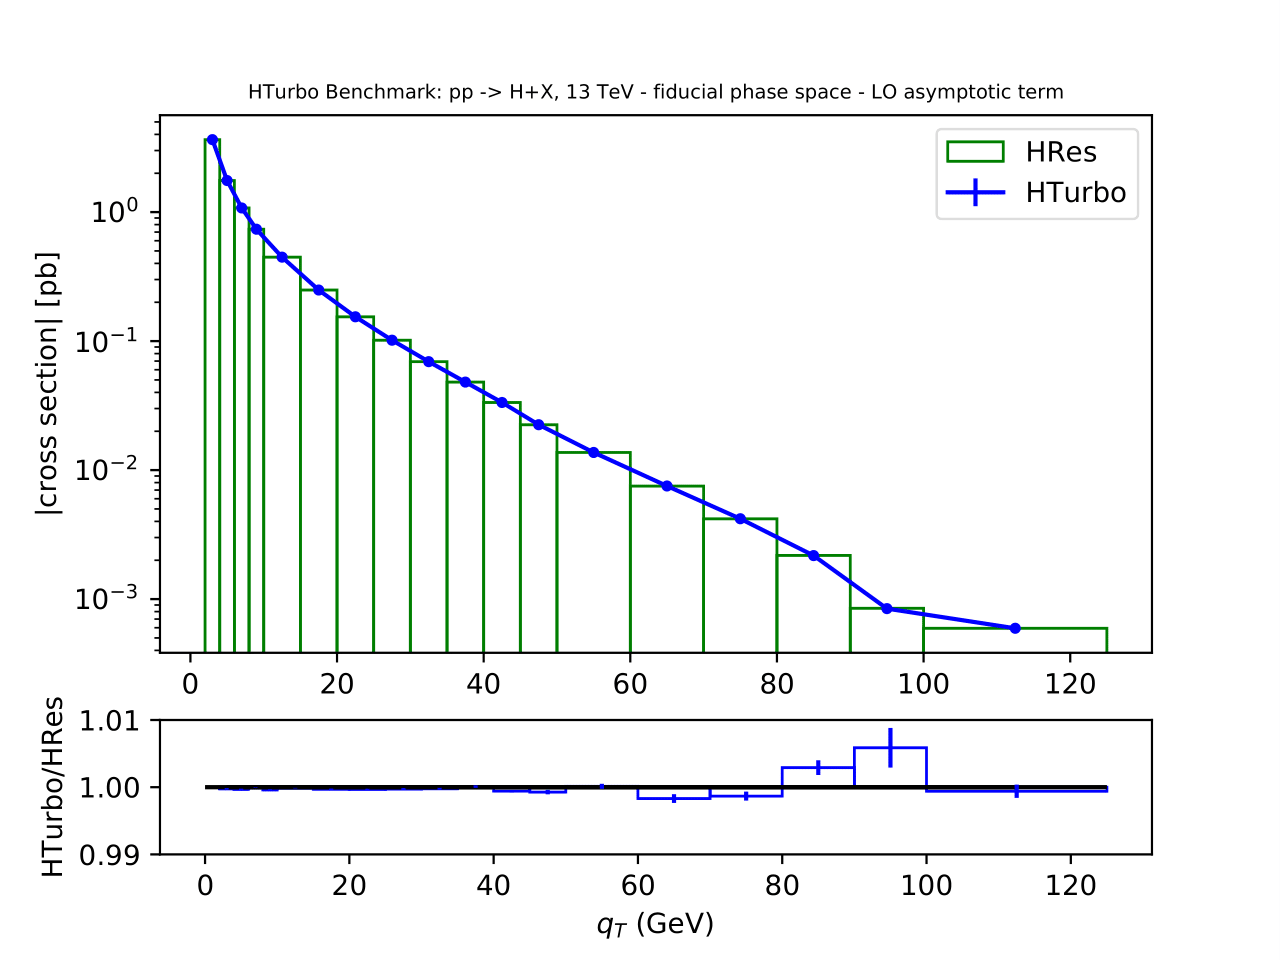
\includegraphics[width = 7cm]{plots/part3/chapter6/nlo-ct-fid-1.png}
		\end{figure}
		
	\end{columns}
	
	\begin{itemize}
		\item Cross section for fully inclusive (LHS) and fiducial (RHS) phase space {\color{darkgreen}$\checkmark$} 
		\item CM energy $\sqrt s = 13$ GeV and PDF set \texttt{NNPDF31\_nlo\_as\_0118 PDF} set
	\end{itemize}

\end{frame}

% Results - Benchmark HRes - NLO asymptotic
\begin{frame}
	
	\frametitle{Results}
	\framesubtitle{Comparison HTurbo and HRes - NLO asymptotic}

	\footnotesize
	
	\begin{columns}
		
		\column{0.5\textwidth}
		
		\begin{figure}
			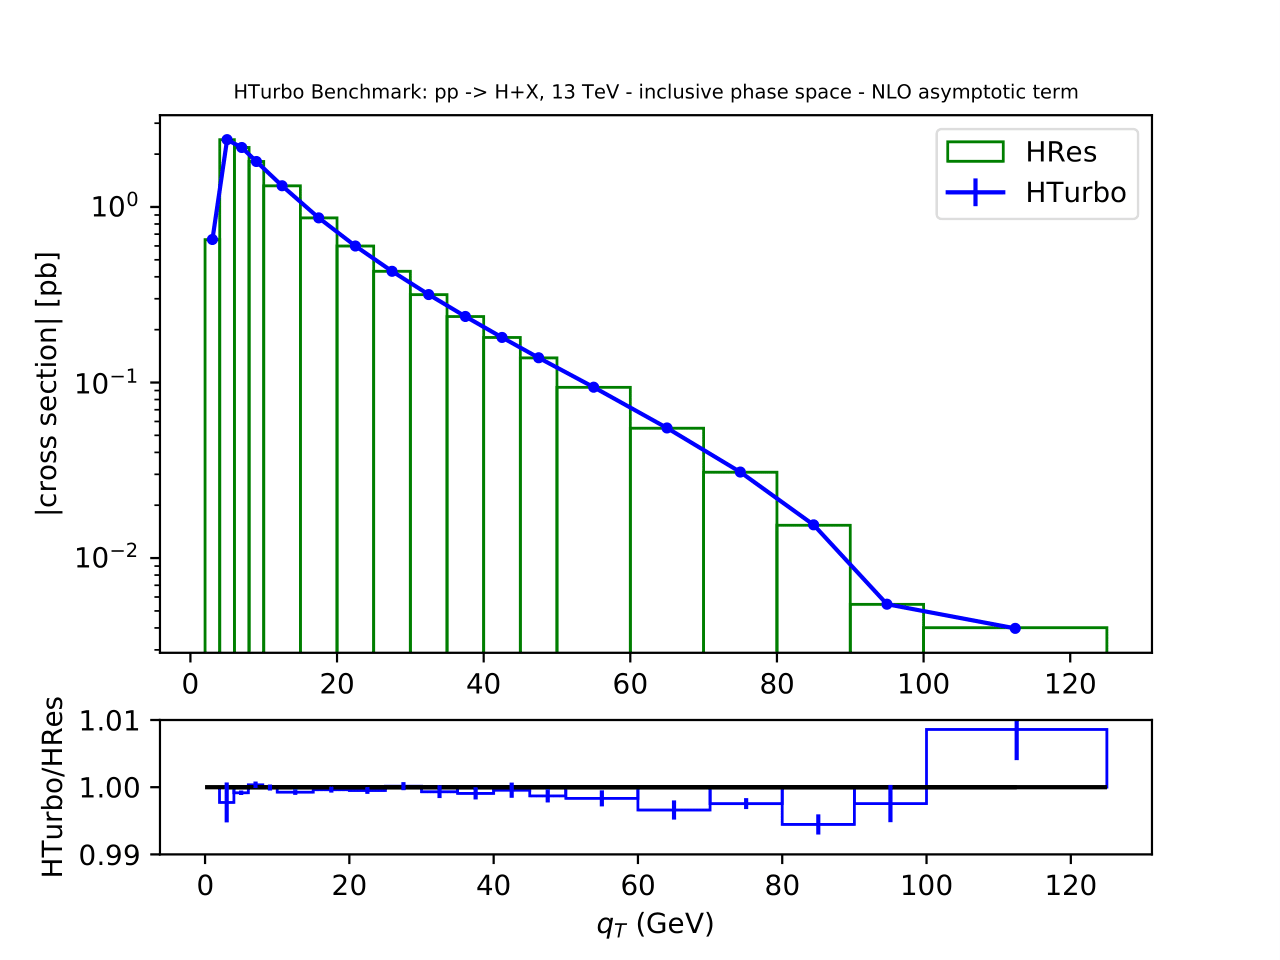
\includegraphics[width = 7cm]{plots/part3/chapter6/nnlo-ct-1.png}
		\end{figure}
		
		\column{0.5\textwidth}
		
		\begin{figure}
			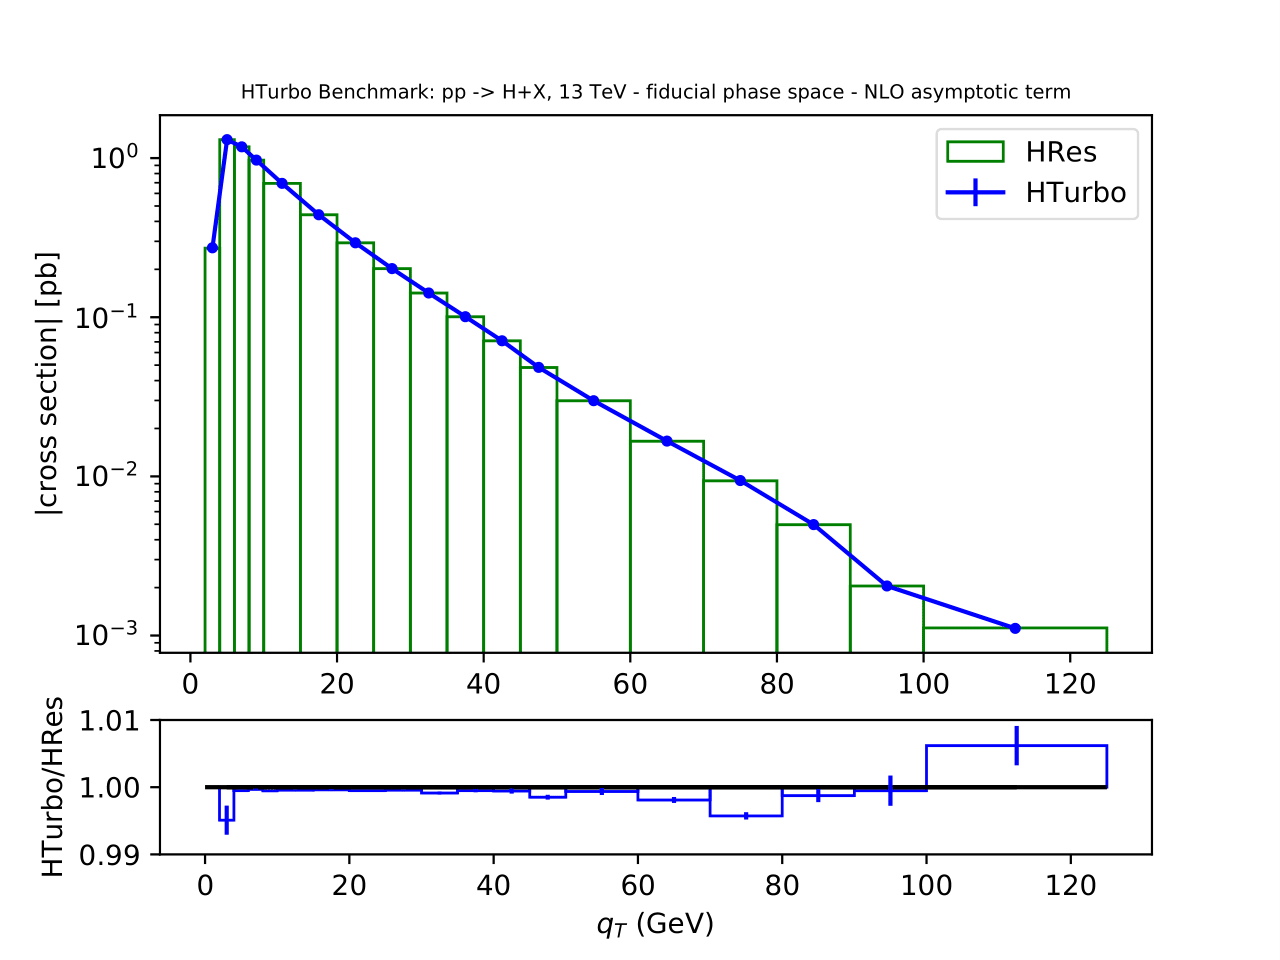
\includegraphics[width = 7cm]{plots/part3/chapter6/nnlo-ct-fid-1.png}
		\end{figure}
		
	\end{columns}
	
	\begin{itemize}
		\item Cross section for fully inclusive (LHS) and fiducial (RHS) phase space {\color{darkgreen}$\checkmark$} 
		\item CM energy $\sqrt s = 13$ GeV and PDF set \texttt{NNPDF31\_nnlo\_as\_0118 PDF} set
	\end{itemize}

\end{frame}

% Results - Benchmark HRes - LO fixed-order
\begin{frame}

	\frametitle{Results}
	\framesubtitle{Comparison HTurbo and HRes - LO fixed-order}
	
	\footnotesize
	
	\begin{columns}
		
		\column{0.5\textwidth}
		
		\begin{figure}
			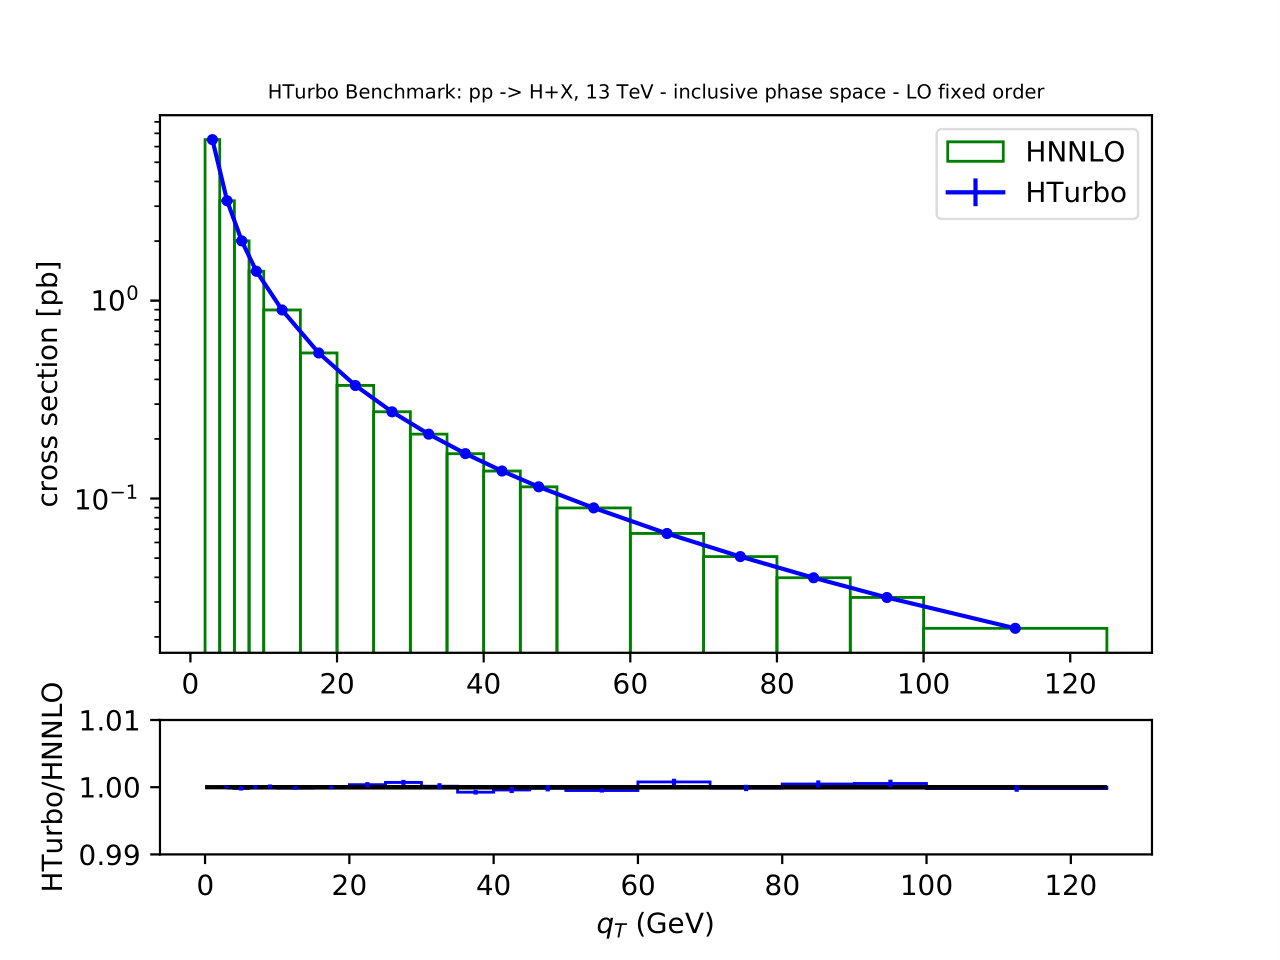
\includegraphics[width = 7cm]{plots/part3/chapter6/nlo-fo-1.png}
		\end{figure}
		
		\column{0.5\textwidth}
		
		\begin{figure}
			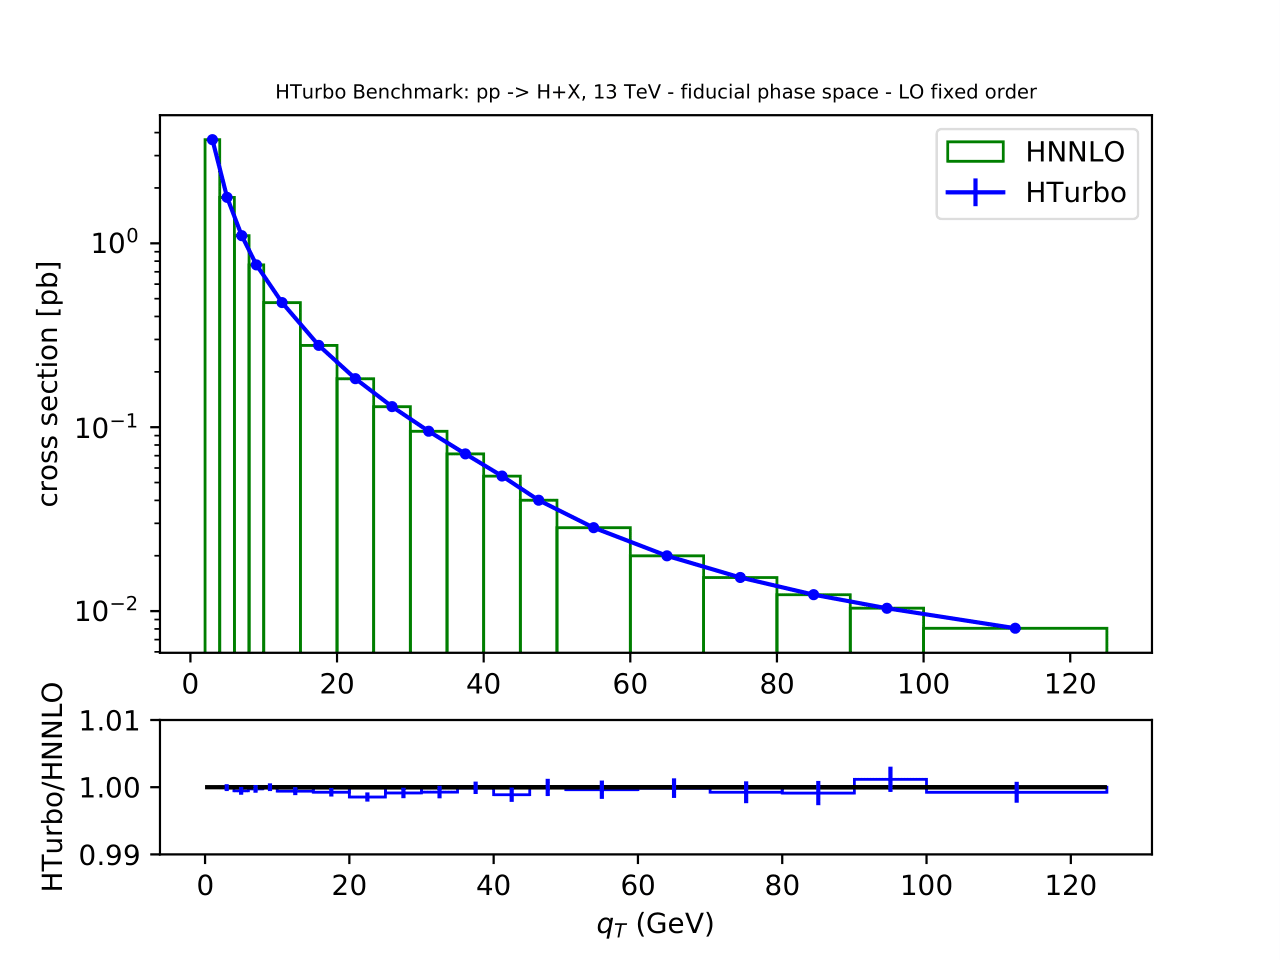
\includegraphics[width = 7cm]{plots/part3/chapter6/nlo-fo-fid-1.png}
		\end{figure}
		
	\end{columns}
	
	\begin{itemize}
		\item Cross section for fully inclusive (LHS) and fiducial (RHS) phase space {\color{darkgreen}$\checkmark$} 
		\item CM energy $\sqrt s = 13$ GeV and PDF set \texttt{NNPDF31\_nlo\_as\_0118 PDF} set
	\end{itemize}

\end{frame}

% Results - Benchmark HRes - LO fixed-order
\begin{frame}
	
	\frametitle{Results}
	\framesubtitle{Comparison HTurbo and HRes - NLO fixed-order}
	
	\footnotesize
	
	\begin{columns}
		
		\column{0.5\textwidth}
		
		\begin{figure}
			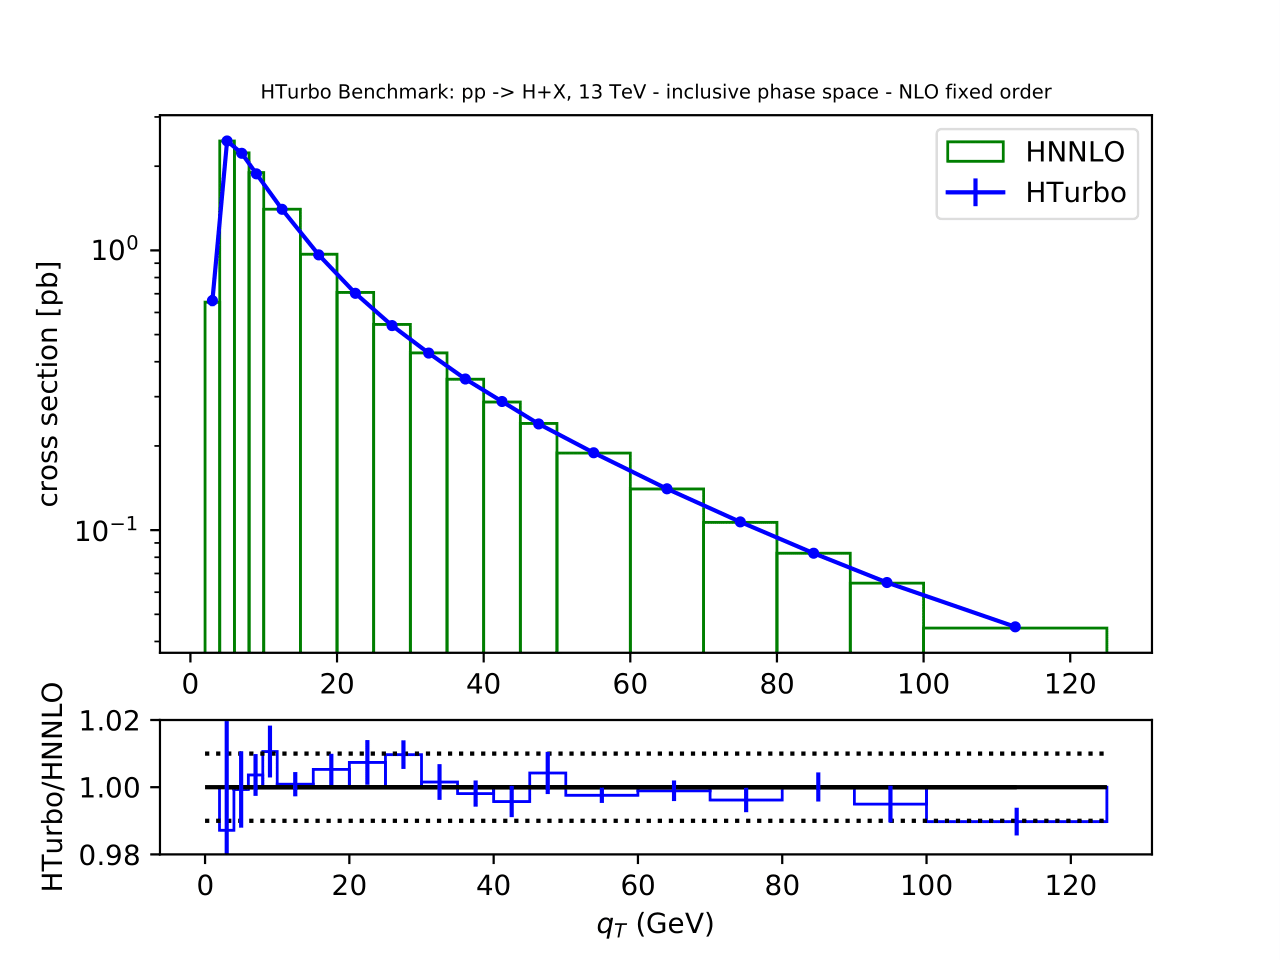
\includegraphics[width = 7cm]{plots/part3/chapter6/nnlo-fo-1.png}
		\end{figure}
		
		\column{0.5\textwidth}
		
		\begin{figure}
			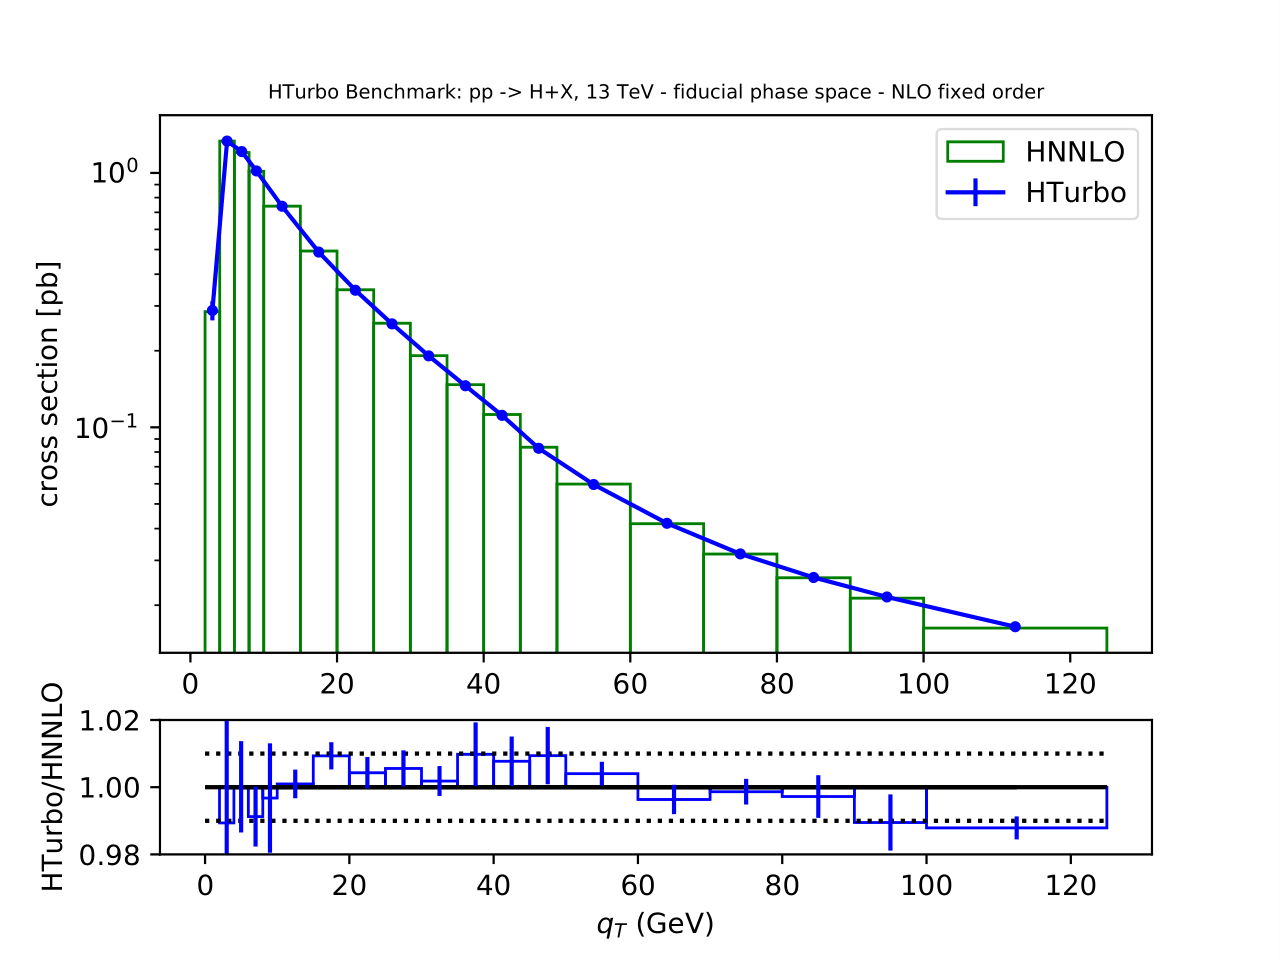
\includegraphics[width = 7cm]{plots/part3/chapter6/nnlo-fo-fid-1.png}
		\end{figure}
		
	\end{columns}
	
	\begin{itemize}
		\item Cross section for fully inclusive (LHS) and fiducial (RHS) phase space {\color{darkgreen}$\checkmark$} 
		\item CM energy $\sqrt s = 13$ GeV and PDF set \texttt{NNPDF31\_nnlo\_as\_0118 PDF} set
	\end{itemize}

\end{frame}

% Results - Speed performance
\begin{frame}
	
	\frametitle{Results}
	\framesubtitle{Speed performance}
	
	\footnotesize
	Test time performance in machine with 3.50 GHz Intel Xeon CPUs:
	
	\vspace{0.5 cm}
	
	\begin{itemize}
		\item HRes NLL resummed $\rightarrow$ 0.5h with with 1\% uncertainty
		\item HTurbo NLL resummed (without multi-threading) $\rightarrow$ 20s with 0.001\% uncertainty
		\item HRes NNLL resummed $\rightarrow$ 48h with 1\% uncertainty
		\item HTurbo NNLL resummed (without multi-threading) $\rightarrow$ 5' with 0.01\% uncertainty
		\item Improvement of {\color{blue}two orders of magnitude in the time performance}
		\item Improvement of {\color{blue}three orders of magnitude in numerical precision}
	\end{itemize}

\end{frame}

% Results - N3LL implementation
\begin{frame}

	\frametitle{Results}
	\framesubtitle{N$^{3}$LL implementation}
	
	\footnotesize
	
	Sudakov factor $\mathcal{G}_{N}$ and hard coefficient $\mathcal{H}_{N}$ can be expanded as perturbative series in $\alpha_{s}$
	\begin{align}
		\mathcal{G}_{N}(\alpha_{s}, L) &= L\;g^{(1)}(\alpha_{s}L) + g^{(2)}(\alpha_{s}L) + \frac{\alpha_{s}}{\pi}g^{(3)}(\alpha_{s}L) + {\color{red} \bigg( \frac{\alpha_{s}}{\pi} \bigg) ^{2}g^{(4)}(\alpha_{s}L)} + ... \nonumber \\
		\mathcal{H}_{N}(\alpha_{s}) &= 1 + \alpha_{s}\mathcal{H}^{(1)} + \alpha_{s}^{2}\mathcal{H}^{(2)} + {\color{red}\alpha_{s}^{2}\mathcal{H}^{(3)}} + ...  \nonumber
	\end{align}
	
	For each new order implement a new factor of $\mathcal{G}_{N}$ and Hard $\mathcal{H}_{N}$
		
	\begin{itemize}
		\item Extend the formalism up to {\color{red}N$^{3}$LO+N$^{3}$LL} accuracy!
		\item Implementation of N$^{3}$LL factors following \\
		\begin{itemize}
			\item {\color{blue} "Anomalous dimension for transverse-momentum resummation", \\
			Li - Zhu, https://arxiv.org/abs/1604.01404},
			\item {\color{blue} "Cusp and collinear anomalous dimensions in four-loop QCD", \\
			Von Manteuffel et al., https://arxiv.org/abs/2002.04617}
		\end{itemize}
	\end{itemize}
	
\end{frame}

% Results - N3LL implementation
\begin{frame}
	
	\frametitle{Results}
	\framesubtitle{N$^{3}$LL implementation}
	
	\footnotesize
	
	\begin{columns}
		
		\column{0.5\textwidth}
		
		\begin{figure}
			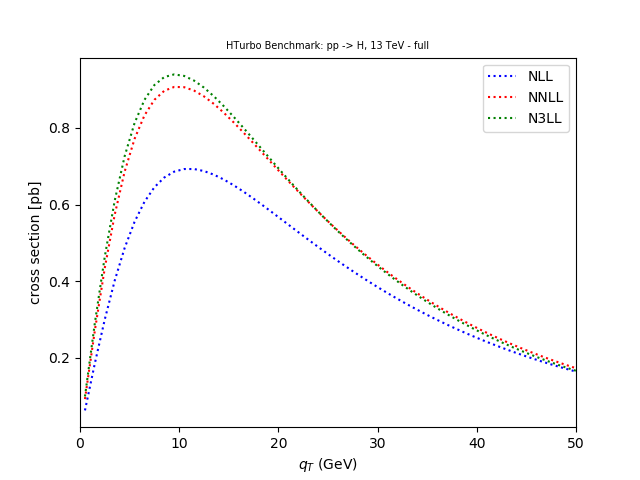
\includegraphics[width = 6cm]{plots/part3/chapter7/hturbo_n3ll.png}
		\end{figure}
		
		\column{0.5\textwidth}
		
		\begin{figure}
			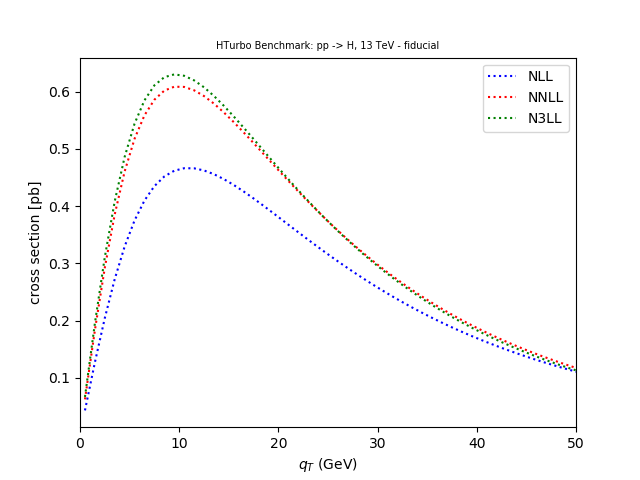
\includegraphics[width = 6cm]{plots/part3/chapter7/hturbo_n3ll_cuts.png}
		\end{figure}
		
	\end{columns}
	
	\begin{itemize}
		\item Cross section for fully inclusive (LHS) and fiducial (RHS) phase space {\color{darkgreen}$\checkmark$} 
		\item Implementation of N$^{3}$LL factors following \\
		{\color{blue}[Li - Zhu, 1604.01404]}, 
		{\color{blue}[Von Manteuffel et al., 2002.04617]}
		\item First implementation of resummed Higgs cross section at N$^{3}$LL accuracy!
	\end{itemize}

\end{frame}

% Summary $\&$ Conclusions
\begin{frame}
	
	\frametitle{Summary $\&$ Conclusions}
	
	\footnotesize
	
	\vspace{2.0 cm}
	
	\begin{enumerate}
		\item Accurate predictions are needed towards the precision era of the LHC
		\item Resummation is needed for describing differential distributions
		\item Fast numerical implementation are needed towards the precision era of the LHC
		\item Developing a novel numerical code, \textbf{HTurbo}, which implements $q_{\perp}$ resummation for Higgs boson production
		\item HTurbo is {\color{blue} faster than any of the existing codes}
		\item HTurbo contains the {\color{blue} first implementation of resummation at N$^{3}$LL accuracy!}
			
		\item Next steps: 
		\begin{itemize}
			\item Add full {\color{blue}N$^{3}$LO+N$^{3}$LL} prediction
			\item Perform phenomenological studies comparing with LHC data
		\end{itemize}
		
	\end{enumerate}

	\vspace{2.0 cm}

\end{frame}

% Conclusions
\begin{frame}

	\center {\color{blue}Thank you!}

	\begin{figure}
		
\includegraphics[width = 2 cm]{plots/final/thinking.png}
	\end{figure}		

	{\small \color{blue} \footnotesize This project has received funding from the European Union$'$s Horizon 2020 research and innovation program under grant agreement No 740006.}

\end{frame}

% Back up
\begin{frame}

	\frametitle{Back up}
	\framesubtitle{Back up}
	
\end{frame}

% Back up
\begin{frame}

	\frametitle{Back up}
	\framesubtitle{General structure of n3fit}
	
	\footnotesize
	
	\begin{figure}[!htb]
		\minipage{0.32\textwidth}
		
\includegraphics[width = 0.5\linewidth]{plots/backup/TF.png}
		\endminipage\hfill
		\minipage{0.5\textwidth}
		
\includegraphics[width = 0.5\linewidth]{plots/backup/Keras.png}
		\endminipage\hfill
	\end{figure}
	
	\begin{itemize}
		\item Use TensorFlow and Keras to determine the PDFs
		\item See paper by S.Carrazza - J.Cruz-Martinez \\
		{\color{blue}"Towards a new generation of parton densities\\ with deep learning models",\\ https://arxiv.org/abs/1907.05075}
	\end{itemize}

\end{frame}

% Back up - TF operator
\begin{frame}
	
	\frametitle{Back up}
	\framesubtitle{General structure of n3fit}
	
	\footnotesize
	
	\begin{figure}
		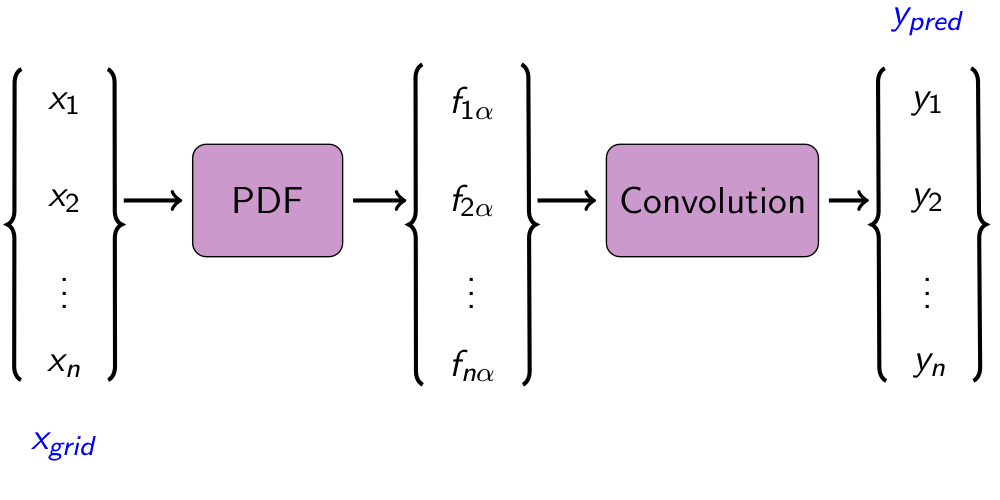
\includegraphics[width = 9 cm]{plots/backup/n3fit1.png}
	\end{figure}	

	\begin{enumerate}
		\item Build a NN to compute $y_{pred}$ observables from a grid of momentum fractions $x_{i}$
		\item Compute loss function by comparing with LHC data
		\item Update values of PDF $\longrightarrow$ {\color{violet} Fit}
	\end{enumerate}

\end{frame}

% Back up - TF operator
\begin{frame}

	\frametitle{Back up}
	\framesubtitle{Operator implementation}

	\footnotesize
	
	\begin{figure}
		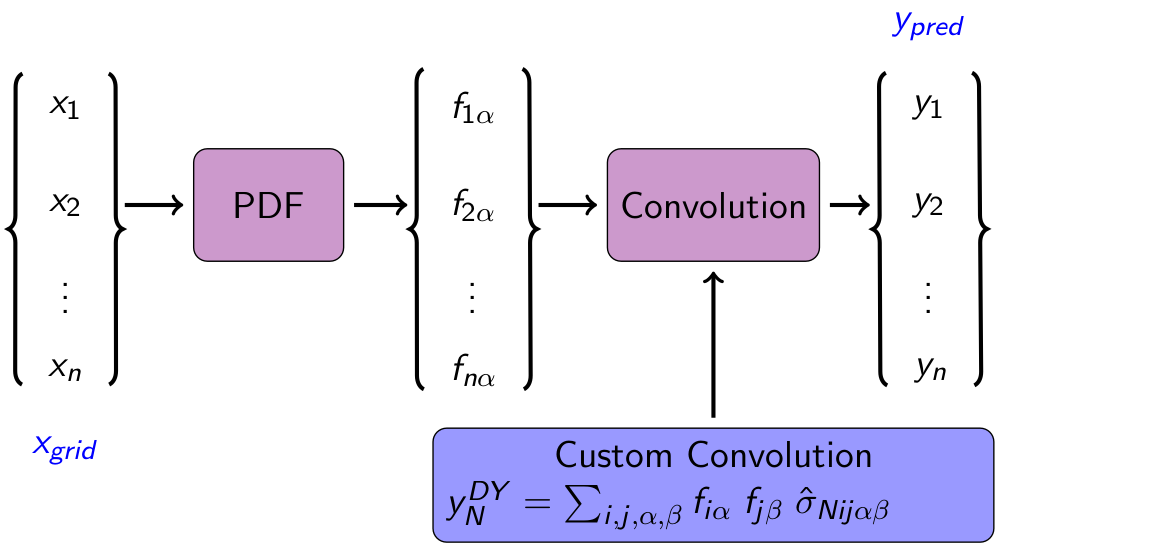
\includegraphics[width = 10.5 cm]{plots/backup/n3fit2.png}
	\end{figure}

	\begin{enumerate}
		\item TF relies in symbolic computation $\longrightarrow$ High memory usage
		\item Implement \texttt{C++} operator replacing the convolution
	\end{enumerate}

\end{frame}

% Back up - benchmark DIS
\begin{frame}

	\footnotesize
	
	\frametitle{Back up}
	\framesubtitle{Benchmark DIS}
	
	{\Large DIS only:}
	\begin{table}
		\centering
		\begin{tabular}{c c c c}
			& TensorFlow & Custom & Ratio \\ \hline
			& 1.9207904 & 1.9207904 & {\color{darkgreen} 1.0000000} \\
			Convolution & 2.4611666 & 2.4611664 & {\color{darkgreen} 0.9999999} \\
			& 1.3516952 & 1.3516952 & {\color{darkgreen} 1.0000000} \\
			\hline
			& 1.8794115 & 1.8794115 & {\color{darkgreen} 1.0000000} \\
			Gradient & 1.505316 & 1.505316 & {\color{darkgreen} 1.0000000} \\
			& 2.866085 & 2.866085 & {\color{darkgreen} 1.0000000} \\
			\hline
		\end{tabular}
	\end{table}

\end{frame}

% Back up - benchmark hadronic
\begin{frame}
	
	\footnotesize
	
	\frametitle{Back up}
	\framesubtitle{Benchmark hadronic}
	
	{\Large DY-like only:}
	\begin{table}
	\centering
	\begin{tabular}{c c c c}
		& TensorFlow & Custom & Ratio \\ \hline
		& 8.142365 & 8.142366 & {\color{darkgreen} 1.0000001} \\
		Convolution & 8.947762 & 8.947762 & {\color{darkgreen} 1.0000000} \\
		& 7.4513326 & 7.4513316 & {\color{darkgreen} 0.9999999} \\
		\hline
		& 18.525095 & 18.525095 & {\color{darkgreen} 1.0000000} \\
		Gradient & 19.182995 & 19.182993 & {\color{darkgreen} 0.9999999} \\
		& 19.551006 & 19.551004 & {\color{darkgreen} 0.9999999} \\
		\hline
	\end{tabular}
	\end{table}

\end{frame}

% Back up - scale variations
\begin{frame}
	
	\frametitle{Results}
	\framesubtitle{N$^{3}$LL implementation}
	
	\footnotesize
	
	\begin{columns}
		
		\column{0.5\textwidth}
		
		\begin{figure}
			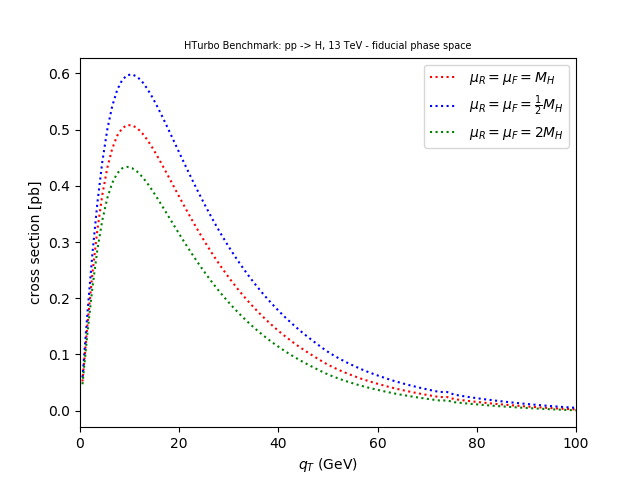
\includegraphics[width = 6cm]{plots/part3/chapter6/hturbo_sv_a.png}
		\end{figure}
		
		\column{0.5\textwidth}
		
		\begin{figure}
			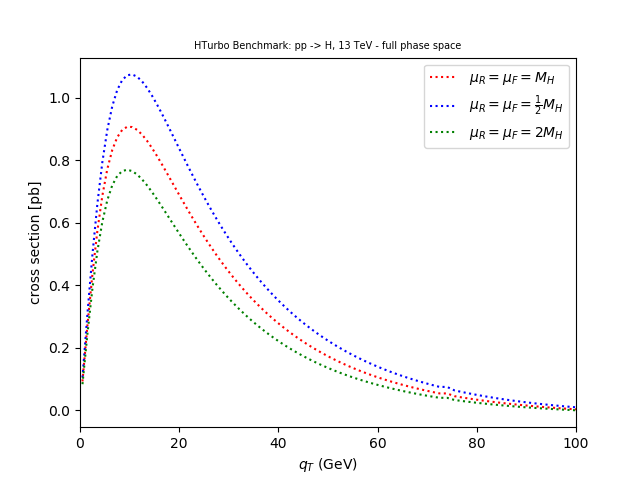
\includegraphics[width = 6cm]{plots/part3/chapter6/hturbo_sv_b.png}
		\end{figure}
		
	\end{columns}
	
	Estimate theory uncertainty:
	
	\vspace{0.5 cm}
	
	\begin{itemize}
		\item i) by performing scale variations on $\mu_{R}$, $\mu_{F}$
		\item ii) by comparing the last two contributions in the perturbative expansion
	\end{itemize}
	
\end{frame}

\end{document}
